\chapter{Introduction\label{cha:introduction}}
%% \ifdraft only shows the text in the first argument if you are in draft mode.
%% These directions will disappear in other modes.

% \ifdraft{State the objectives of the exercise. Ask yourself:
%   \underline{Why} did I design/create the item? What did I aim to
%   achieve? What is the problem I am trying to solve?  How is my
%   solution interesting or novel?}{}

% The object of the project is to be able to monitor cetacean traffic around Iceland.
% This could help tourism companies relating to whale watching. 
% Could also be extended to whale researchers.


Humans have caused increased pressure on animals whether that be land or sea creatures.
Keeping track of the creatures is vital to ensure their health and survival for the future.
This can be done by population assessments, which can show if the specific species is in an upsurge or declining in terms of numbers.
For fish and cetaceans, there are several ways to achieve this for example the animal can be tracked via Global Positioning System (GPS) tracker or the animal is visually sighted by the use of a boat or aircraft.
These methods are however time-consuming and require a lot of manpower.
To plant a tracker on the animal it must first be found and captured to attach the tracker and the latter method requires researchers to actively search the animal, which is heavily reliant on favorable sea conditions etc.
There are however methods available that rely on acoustic surveys to monitor cetaceans which enables researchers to not only explore the surface of the ocean but also beneath the waves.
These surveys can be done in several ways.
One method involves dragging an array of hydrophones and record the vocalization data.
The second is to mount hydrophones into the bow of the ship and record the vocalization data.
This method however can not be used when recording low-frequency sounds, due to the noise created by the ship and water flow as well as still requiring researchers onboard ships actively looking for animals.
The third method and the one this thesis will focus on is using a buoy to passively gather cetacean vocalization.
Where a hydrophone and a recording device are attached to a buoy that moored in place and sets on recording passively that location without the need of external help and maintenance.

The buoy must be self-sufficient and able to stay out at sea for long periods at a time to serve its function.
This means that all the electronics onboard will need to be powered by the buoy.
It also has to be able to record cetacean vocalization and transmit the data onshore.
So that marine researchers can study the data or even whale watching companies in the tourism industry can play cetacean vocalizations in the fjords.
This means the passive sound gathering buoy can be separated into three different projects, power production, sound gathering and data transmission onshore.
This thesis will focus on developing a device for the cetacean vocalization recording.

This function will be implemented using a Teensy 3.5 microcontroller.
A hydrophone will be used to sense the sound waves generated by the cetacean vocalization which have an extremely wide frequency range of a few Hz to hundreds of thousands of Hz echolocation signals. This project will have therefore gather signals in the range of 10Hz to 100kHz, at at least 16bits resolution for high-quality audio.
The electrical circuit will consist of a preamplifier, filter, analog to digital converter and SD card for data logging.





\section{Project Goals}

The objective of the project is to create a relatively small, low cost and a low-maintenance device capable of recording cetacean vocalization and transmitting the data onshore.
The design criteria for the project are as follows.
The total power consumption of the system should be less than 10 watts. 
The device should be relatively small and lightweight, so it is deployable by one person.
The device should last 6 months at a time.
Maximize the frequency at which the device can record.
%Be able to gather data of signal ranging from 10Hz to 100kHz. \fxfatal{Skoða aðeins betur}
\clearpage

\section{Background}

Considerable cetacean preservation efforts have been carried out for the past decades.
In 1946 the International whale commission, which is a global body with the goal of conservation of whales and currently has 88 member governments from all over the world.
Which is a global organization to conserve and manage whales and it currently has 88 countries signed to the committee \cite{noauthor_iwc_nodate}.

Many methods have been used to monitor the population of cetaceans.
These methods range from very active hands-on surveys where Marine Mammal Observers (MMOs) capture, examine, mark and then let the animal go to be recaptured in the future.
To a more passive acoustical survey where hydrophones are utilized to listen in on cetaceans.

%https://www.sciencedirect.com/science/article/pii/S0003347216301452#:~:text=We%20describe%20several%20methods%20developed,high%2Dresolution%20acoustic%20recording%20tags.

\subsection{Visual surveys}% and photogrammetry 

Visual surveys are generally carried out by the use of boats, helicopters or airplanes.
Trained marine researchers use high-power binoculars to search for cetaceans breaching the surface of the ocean.
Once the cetacean is sighted it is categorized accordingly with regards to the study.
Immense data can be extrapolated from such research as the location of the sighting, the species sighted, group size to name a few\cite{campbell_inter-annual_2015}.
However several factors might limit or stop a visual survey such as sea conditions, visibility, the behavior of the animal.
As well as the countless other animals that could lie just beneath the surface out of MMOs sight.

\subsection{Hands-on surveys}

This method utilizes animals that are caught and released, animals that are being cared for and animals that have become incapacitated by beaching. 
Animals that are caught are identified, which can be done by taking photographs of markings or identifying features, that in the future could be used to identify the animal if it is ever recaptured.
This is known as photo-identification\cite{booth_methods_2020}.
This approach has been utilized to gain a further understanding of the population and health of cetaceans.

Individual tracking surveys are similar in the fact that the animal is captured and released in the same manner.
However, instead of taking photographs of it before releasing it, the animal would have a GPS tracker attached to it. 
Which has been utilized for research into acquiring data regarding behavior and responses of disturbance sources as well as data on the animals travel and habitat patterns. 
Depending on what the researcher wants to get data on will dictate whether or not the GPS tracker is added on to the animal\cite{booth_methods_2020}.



\subsection{Acoustic surveys}

Methods previously mentioned rely heavily on favorable conditions regarding sea conditions, weather and visibility since the MMOs need to be able to spot the cetaceans.
There are different methods to conduct the surveys, which can fall into one of two categories either active or passive.
Active acoustic monitoring (AAM) includes systems such as fish sonars and echo sounders. 
Cetaceans are detected with target reflection instead of vocalization \cite{pyc_evaluation_2015}.
Passive acoustic monitoring (PAM) relies on the use of hydrophones, where cetacean vocalizations are recorded and studied.\\
\indent There are several methods to choose from when conducting a PAM.
The first method involves towing an array of hydrophones behind a vessel at sea such as a ship and recently autonomous platforms have been utilized instead\cite{baumgartner_diel_2008} .
This however still requires favorable sea- and weather conditions, as well as when a ship is used there still needs to be active MMOs on board.
Another is to mount hydrophones in the bow of the ship.
This method is however limited frequency range due to the noise created by the ship bow and water flow\cite{rankin_acoustic_2008}.
The third is to have a fixed device, that has hydrophones and can either store vocalization data on the device itself or transmit the data directly onshore to researchers.
These devices are generally capable of long-term unmanned monitoring and can be a quite cost-effective alternative.
All three methods can eliminate most if not all of the previously described problems that can occur with visual surveys.



\subsection{Devices currently available}
\subsubsection{$\mu$RUDAr-mk2}

Devices such as the $\mu$RUDAR-mk2 as seen in \textit{Figure~\ref{fig:uRUDAR}}, is a product from Cetacean research technology that offers a remote fixed monitoring system.
It has the ability to remote autonomous recording.
WiFi recording control and data transmission capability.
The device can record up to 24-bit/96kHz and 45kHz bandwidth and up to 16.5 days of continuous recording time\cite{computing_microrudar_nodate}.
This device however relies on battery power and cant generate electricity and therefore has limitations on deployment time.

\begin{figure}[h]
    \centering
    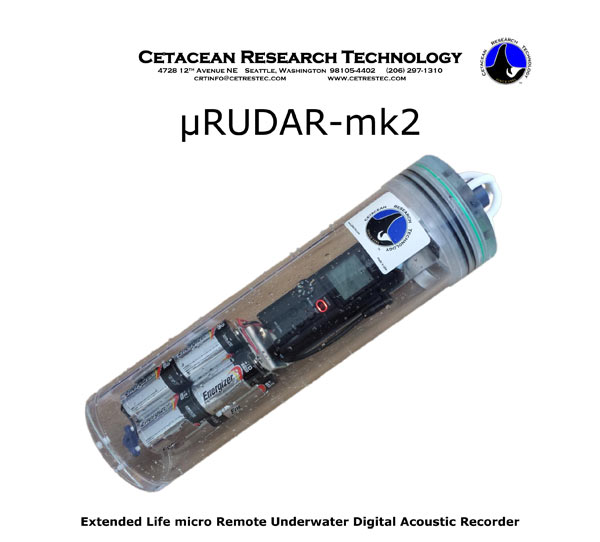
\includegraphics[width=0.70\textwidth]{graphics/uRUDAR-mk2.jpg}
    \caption{uRUDAR-mk2 fixed monitoring device\cite{computing_microrudar_nodate}}
    \label{fig:uRUDAR}
\end{figure}

\subsubsection{RUDAR (Remoter Underwater Digital Acoustic Recorder)}
Another recording device from Cetacean research technology is the RUDAR (Remoter Underwater Digital Acoustic Recorder), seen in \textit{Figure~\ref{fig:Rudar}}. 
It is an autonomous recording device that is small enough to be hand deployed from a small boat.
The recording system uses the ST400 mobile data recorder and sound level monitor. 
The system has a working depth of 1.5-3.5km it can record from 4 hydrophones at 24-bit resolution.
The data is written to an internal hard drive and can record 2 independent schemes and sample rates at the same time \cite{cetacean_research_technology_rudar_2021}.

\begin{figure}[h]
    \centering
    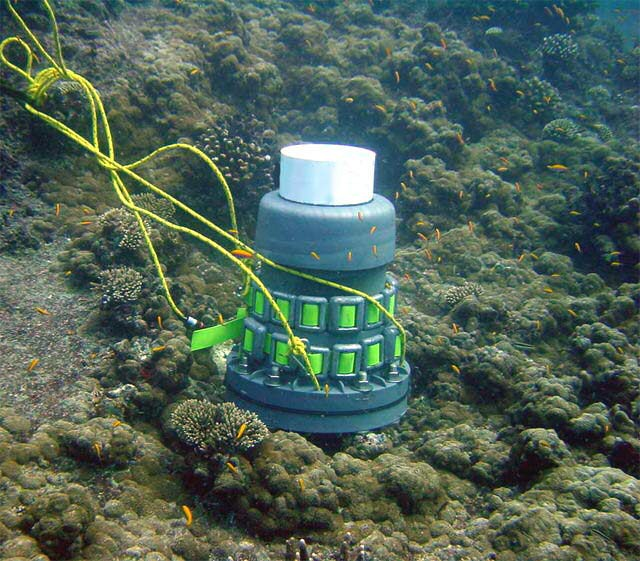
\includegraphics[width=0.70\textwidth]{graphics/Rudar.jpg}
    \caption{RUDAR recording device \cite{cetacean_research_technology_rudar_2021}}
    \label{fig:Rudar}
\end{figure}

%\fxfatal{TALA KANSKI UM F-pod hér \cite{noauthor_f-pod_nodate}}

\subsubsection{Persistent near real‐time passive acoustic monitoring for baleen whales from a moored buoy.}
A system has been developed for the United States Coast Guard that is capable of long-term remote deployment. 
The system consists of a moored buoy that can provide data collection and transmission.
It has passive acoustic instruments such as digital acoustic monitoring(DMON) and a low-frequency detection and classification(LFDCS) firmware.
The system has three hydrophones and a programmable Texas Instruments TMS320C55 digital signal processor (DPS) as well as GPS.
The firmware is used to build a spectrogram of the recorded sounds when the mooring is recovered.
An example of which can be seen \textit{Figure \ref{fig:SpectoExamp}}.
It then classifies the sound calls by comparing attributes of the pitch track to known call types. 
The mooring hardware of the surface buoy is used for power delivery as well as data transmission. 
The system has an internal battery capacity of 450 Ah. 
%The audio is recorded with a sampling frequency of 2kHz. 
It is designed to operate for 1 year at a time has a maximum data transfer rate of 8Kb per hour through Iridium global communication system \cite{baumgartner_persistent_2019}.

\begin{figure}[h]
    \centering
    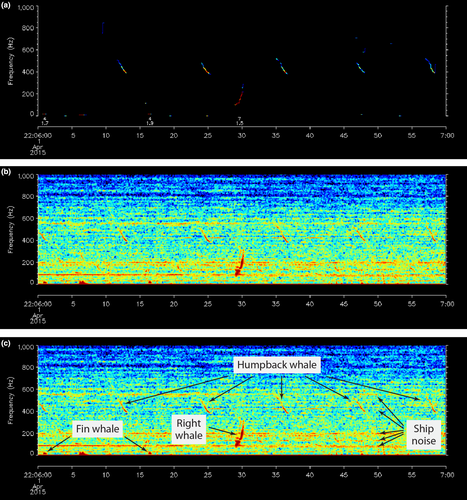
\includegraphics[width=0.60\textwidth]{graphics/spectogram.png}
    \caption{Spectogram that can be produced once the mooring is recovered.
    (a) In near-real time detection information (b) spectogram for a the given time period seen in (a) at 2000Hz sampling rate (c) addition of annottations of sound source to spectogram seen in (b)\cite{baumgartner_persistent_2019}}
    \label{fig:SpectoExamp}
\end{figure}

The setup of the system can be seen in \textit{Figure~\ref{fig:DMON/LFDCS}} from the moored surface buoy at the top, to the monitoring device at the bottom of the ocean.

\begin{figure}[h]
    \centering
    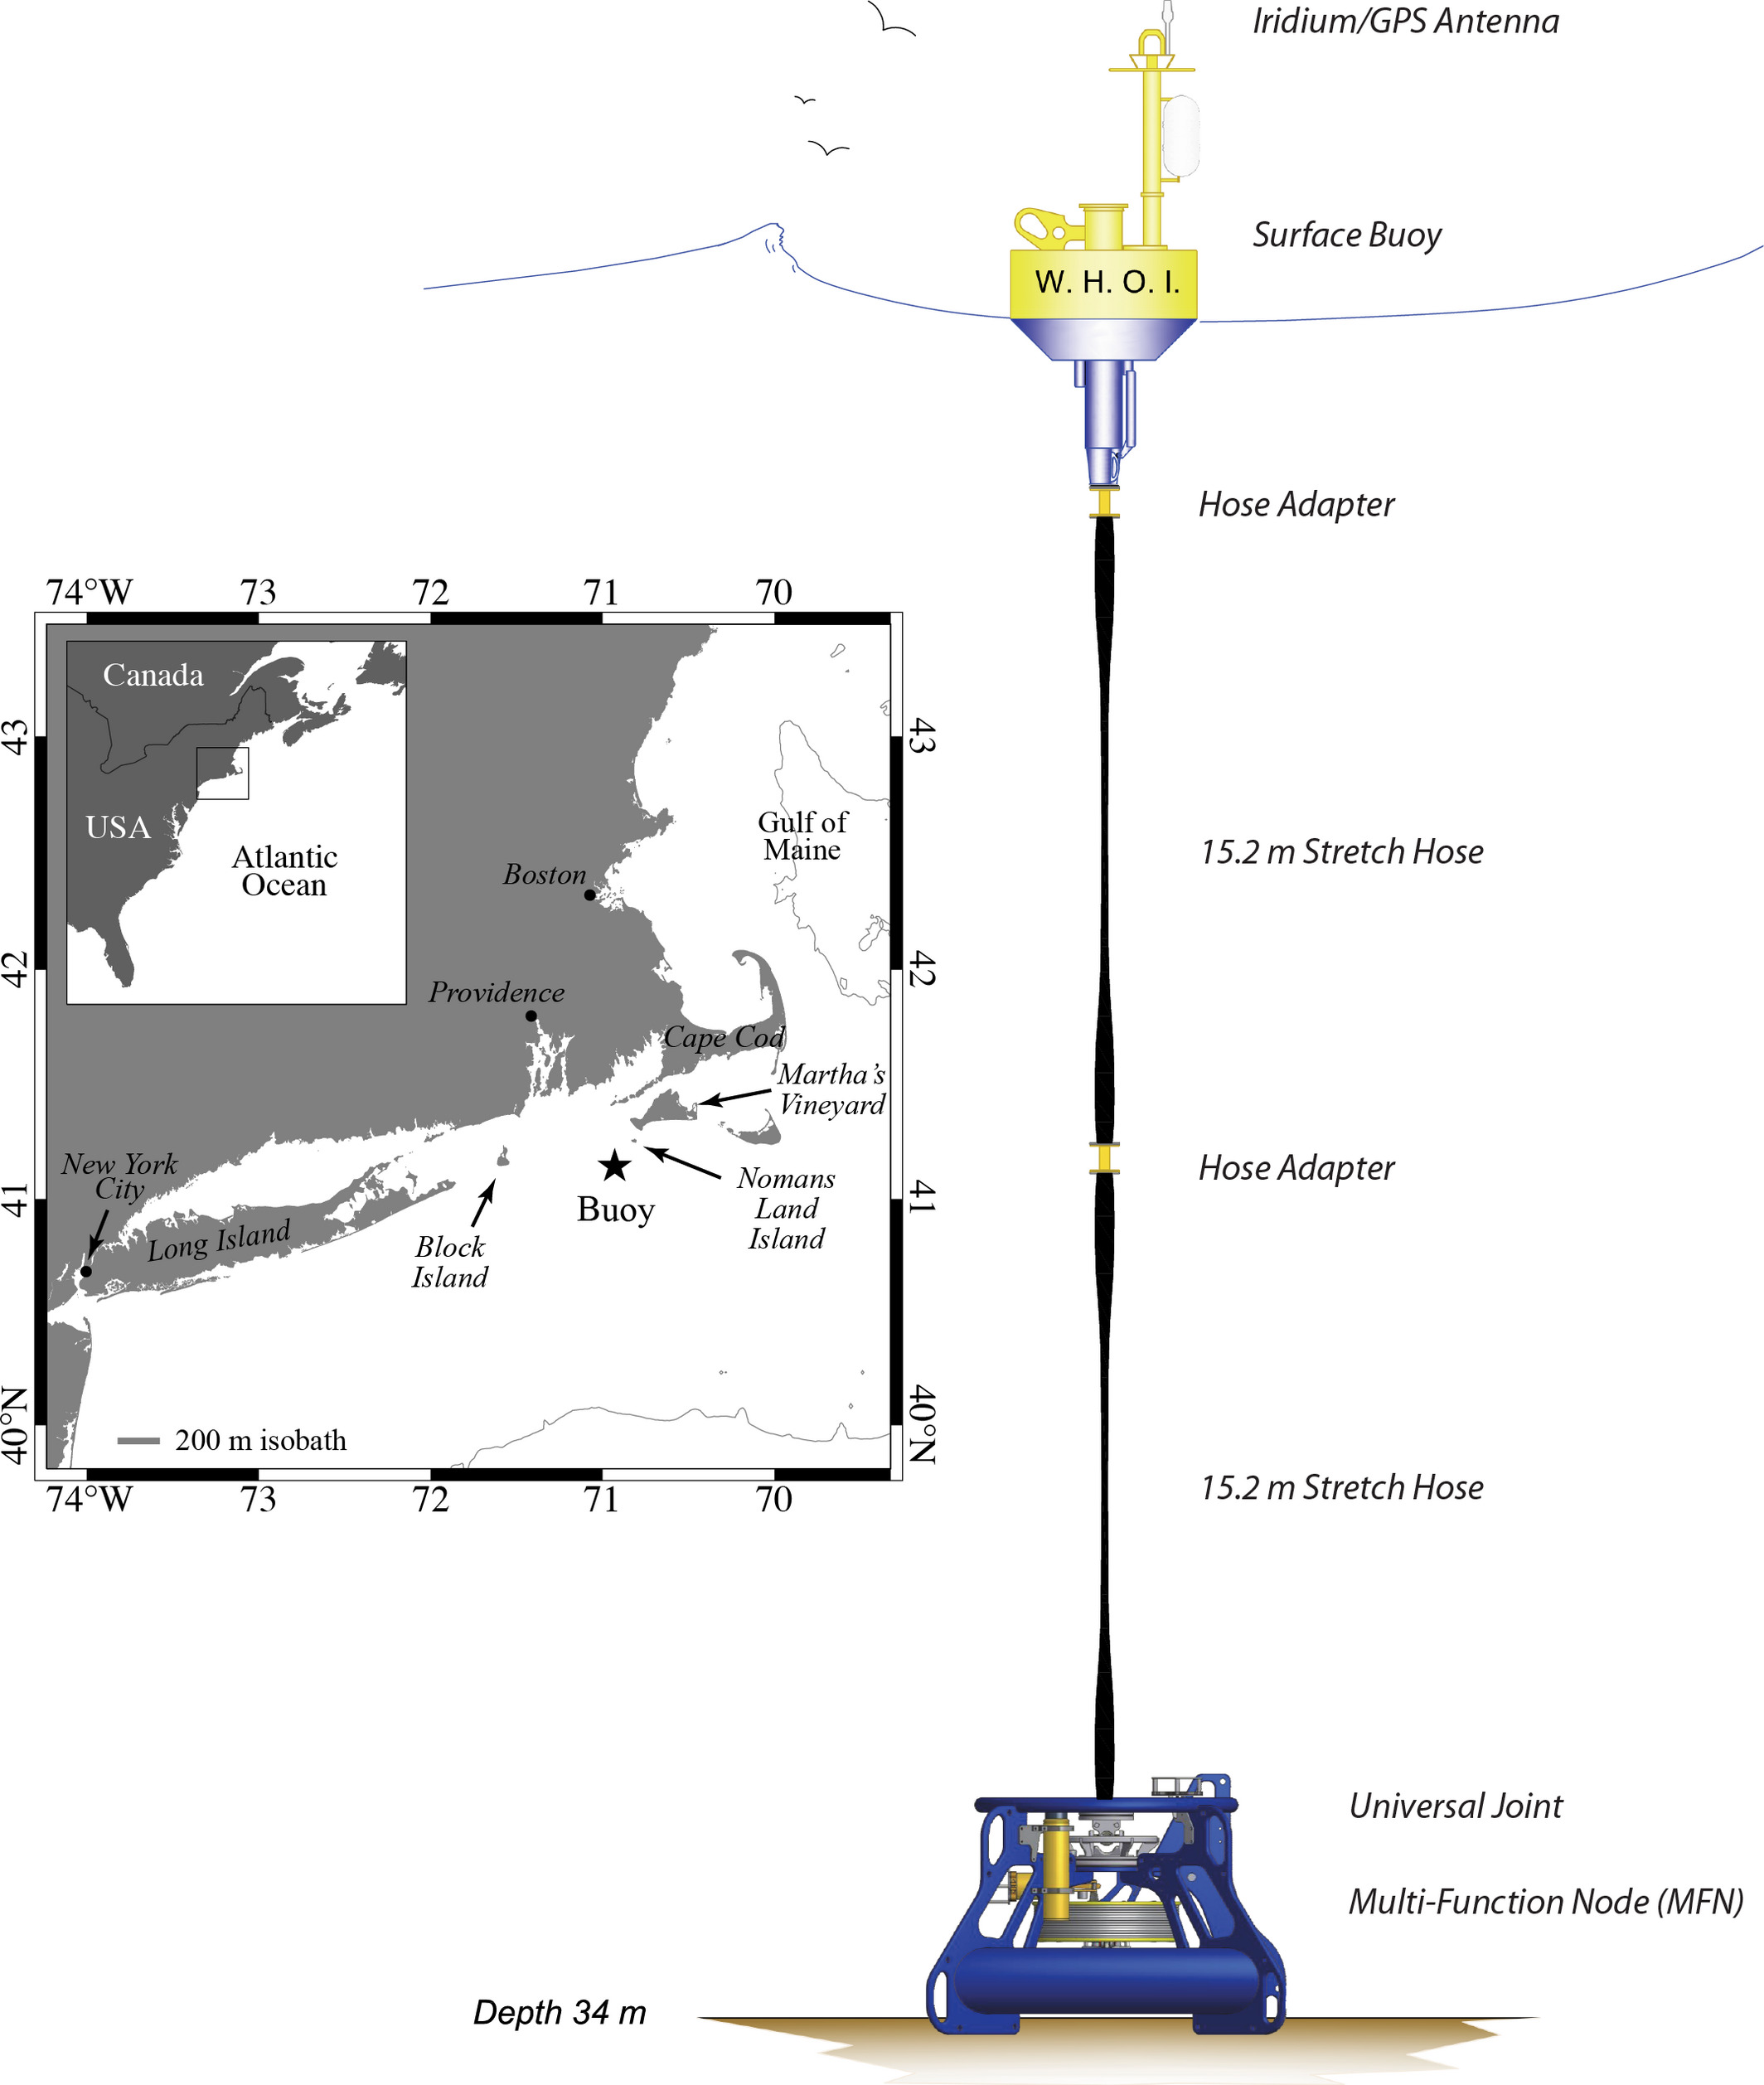
\includegraphics[width=0.70\textwidth]{graphics/DMONbuoy.jpg}
    \caption{A moored buoy using DMON/LFDCS systems, designed for 1 year deployments\cite{baumgartner_persistent_2019}}
    \label{fig:DMON/LFDCS}
\end{figure}

\clearpage


\subsection{Cetacean vocalization}

Many different species of cetaceans can be found near Iceland.
There are at least 12 species that roam Icelandic oceanic waters.
Among which are most frequently spotted are harbor porpoise, white-beaked dolphins, minke whales and humpback whales \cite{user_whales_nodate}.
Sound is used by cetaceans for various purposes the low-frequency sounds are used for communication and high-frequency prey hunting, predator avoidance, as well as echolocation for navigation \cite{nowacek_studying_2016}.
Each species can vocalize different sounds.
The sounds can be described as moans, calls, clicks, shrieks and more\cite{greenhow_hearing_nodate}.
%Cetaceans use these sounds to low-frequency sound for communicating to one another to creating high frequencies echolocation sounds for hunting their prey\cite{greenhow_hearing_nodate}.
\textit{Table \ref{Tab:WhaleHz}} shows the type of sound, the frequency range of the sound, the dominant frequency of the sound and the source level of each sound for its respective species.

Cetaceans produce vocalization and echolocation sounds with a wide bandwidth, or 2 - 150kHz as seen in \textit{Table \ref{Tab:WhaleHz}}.
In comparison, humans have a vocalization range of up to 5kHz and a hearing range from 16Hz - 20kHz \cite{monson_perceptual_2014}.
The vocalization can be so powerful that the low-frequency sounds might be able to travel thousands of kilometers\cite{nowacek_studying_2016}.
The energy of sounds from for example killer whales, in calm seas can travel up to 25.9km.\cite{miller_diversity_2006}.



\subsection{Audio}

\subsubsection{Sound waves}

Sound is a mechanical vibration, which results in an oscillating wave.
The wave causes a change in the pressure of molecules.
The wave can travel through gasses, liquids and solids.
It occurs when objects vibrate, such as a diaphragm of a speaker or a vocal cord of a human.
It is a wave that has a frequency and amplitude, which determines the type of sound and the intensity of the sound.
Sound waves behave very differently in liquid and air.
In liquids such as seawater, several things affect sound propagation.
Such as the sound can bounce off particles or other sea creature and even the bottom and the surface of the sea which causes reflection to the sound waves and cause energy loss.
Finally and the largest factors are depth, salinity and temperature of the water.
These factors can distort the sound and create transmission losses\cite{noauthor_sonar_nodate}.
The speed of sound is quite different whether it is traveling in the air or the ocean.
Speed of sound for example in 20°C air is roughly 343m/s, while in the ocean it a lot faster and can vary around 1500m/s depending on the temperature, pressure and salinity of the ocean. 

\begin{figure}[h]
    \centering
    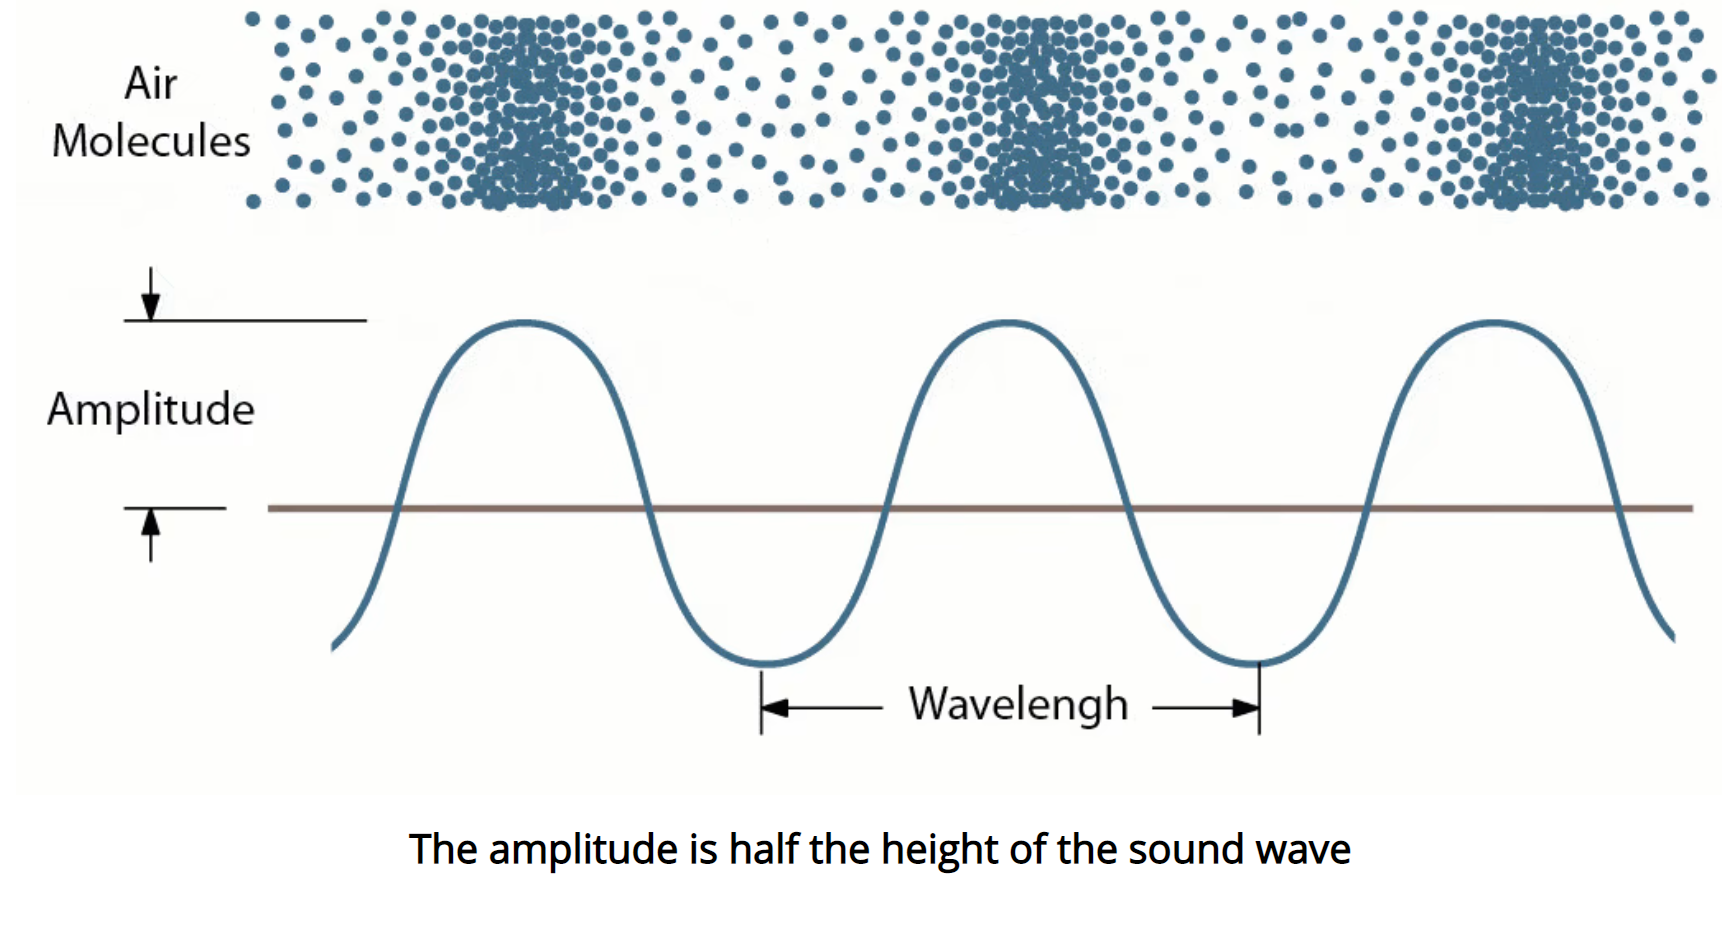
\includegraphics[width=0.70\textwidth]{graphics/soundwaves.png}
    \caption{How molecules react to sound waves \cite{noauthor_what_nodate}}
    \label{fig:SoundWaves}
\end{figure}

\subsubsection{Digital audio recording}\label{sec:DigitalAudiRec}

%https://documentation.meraki.com/MR/WiFi_Basics_and_Best_Practices/Signal-to-Noise_Ratio_(SNR)_and_Wireless_Signal_Strength#:~:text=The%20SNR%20is%20the%20difference,signal%20and%20the%20noise%20floor.&text=For%20example%2C%20if%20a%20client,dB%20for%20this%20wireless%20connection. - SNR

Audio recording is the recreation of sound waves, which can either be analog- or digital recorded.
Digital recording is the process of converting analog sounds, which means converting the analog signals from a microphone to a digital format. 
This is done by representing the audio signal with binary numbers, which represents the amplitude or intensity of the sound and then sampling or recording that sound at a given time interval.
The greater the resolution the less noise is being recorded.
Resolution is determined by the number of bits used to record a signal and deter the precision of the measurements, it is the smallest incremental voltage change that can be recognized.
For example, if a signal had a voltage range from 0 - 3.3V and it was being recorded at 16bits the voltage resolution would be $\frac{3.3V}{2^{16}} = 50\mu V/bit$.
Which would mean that the recording could in theory have $50\mu V$ increments in representing the signal.  
While an 8bit resolution only yields $\frac{13mV}{bit}$, meaning the higher the resolution, the more precise the measurement values are.
However, with more bits come more data rate and higher storage requirements.

\begin{equation}
    Data Rate = \frac{Bits}{8} * Sampling Rate * Number of channels 
    \label{eq:dataRate}
\end{equation}

Data rate can be calculated using \textit{Equation~\ref{eq:dataRate}}.
Where bits are the ADC resolution, sampling rate is the sampling frequency in Hz and the number of channels is how many signals are being recorded.
The data rate can then be used to determine the amount of storage needed.
Nyquist-Shannon theorem is in digital recording to determine the minimum sampling rate needed to reconstruct the analog signal.
The theorem proves that if the sampling frequency is twice the frequency of the highest frequency of the input analog signal, the signal can be recreated exactly.% \cite{bartlett_practical_2016}.
So in theory, since humans have a hearing range of up to around 20kHz, to reconstruct all signals that are audible to humans, the sampling rate needs to be at least 40kHz.
For example on CDs the quality of the recording is 44.1kHz/16bits, in DVDs it is 96kHz/24bits and for high-end audio recording, it can go to 192kHz/24bits.
The oversampling can improve the recording for more accurate recording.
But oversampling is a term used for when the sampling frequency is of a higher rate than the Nyquist-Shannon theorem states  \cite{bartlett_practical_2016}.
If for example a sampling frequency of 200kHz was used when the signal being recorded was 20kHz it would be considered 5x oversampling.
The frequency that controls the ADC conversions also has to be precise.
If the timing of the samples is unstable it is called jitter, which is the standard deviation from the mean of the clock used to control ADC conversions.
The difference in decibel between the signal and the noise floor is called signal to noise ratio (SNR), meaning the difference between the input signal and the no signal is the SNR.
For cleaner sounds, meaning less noise is audible and more of the actual signal of interest, the higher the SNR.
Generally it is considered fair if the SNR is 60dB, good if SNR is 70dB and great if its 80dB or more \cite{bartlett_practical_2016}.


%\section{Device hardware}

%\textbf{FARA 'I GEGNUM VERKEFNI SEM AÐRIR HAFA GERT RUNNA ÞAU OG TALA UM NIÐURSTÖÐUR OG DÆMA HVÐ VIRKAR HVAÐ EKKI OG AFHVERJU ÞETTA GETUR VERIÐ EH APPENDIX DÆMI}

\subsection{Hydrophone}

Hydrophones are devices specially designed for underwater sound recording.
One of the earliest known examples of a hydrophone was made by stretching a membrane tightly over the end of a tube, one end of the tube is placed underwater while the other end is placed to the observer's ear \cite{wood_a_b_textbook_1946}. 
Modern hydrophones are mainly based on piezoelectric transducers.
These hydrophones have been used since the early stages of world war 1.
Paul Langevin developed the first piezoelectric hydrophone, which was intended to be used for the detection of submarines.
A vacuum tube amplifier in combination with a piezoelectric material to be used as a transducer signal\cite{van_der_kloot_great_2014}.

When choosing a hydrophone it is important to look at a few specifications in the datasheet of the hydrophone. 
Such as the open circuit receiving response (OCRR), which is what the transducer outputs in terms of dB re 1V/$\mu$Pa.
As well as the frequency range that the hydrophone can receive and how much amplification it needs for different applications.
Also, some things to consider are things like
%Which is a function of frequency and expressed in terms of dB re 1V/$\mu$Pa.
sound intensity level (SIL) is the intensity of the sound at the transducer and is expressed in terms of dB re $\mu$Pa.
As well as transmitting voltage response (TVR) is the output voltage of the SIL at 1m range from the transducer and is expressed in terms of dB re $\mu$Pa/1V @ 1m \cite{ethem_mutlu_sozer_underwater_nodate}. 
Usable frequency of the hydrophone, directional patterns of the hydrophone and if it applies the nominal capacitance of the hydrophone are also important factors. 
If for example the CRT C57 hydrophone was chosen, specifications can be seen in \textit{Table \ref{Tab:CRT57Hydrip}}.


\begin{table}[h]\caption{Specifications of CRT C57 hydrophone range \cite{computing_c57_nodate}}.\label{Tab:CRT57Hydrip}
\centering
\begin{tabular}{|r|c|c|}
\hline
\multicolumn{1}{|c|}{\textbf{}} & C57 / C57X & C57RS/C57XRS \\\hline
{\begin{tabular}[c]{@{}r@{}}Linear Frequency Range \\ (±3dB) {[}kHz{]}\end{tabular}}      & 0.015 to 45         & \begin{tabular}[c]{@{}c@{}}0.015 to 50\&\\ 124 to 250+\end{tabular} \\ \hline
{\begin{tabular}[c]{@{}r@{}}Usable Frequency Range \\ (+3/-12dB) {[}kHz{]}\end{tabular}}  & 0.008 to 100        & { 0.008 to 77 \& 96 to 250+}                    \\ \hline
{\begin{tabular}[c]{@{}r@{}}Transducer Sensitivity* \\ {[}dB, re 1V/µPa{]}\end{tabular}}  & -187                & { -200}                                         \\ \hline
{Preamplifier Gain {[}dB{]}}                   & 20 / 33             & { 20 / 33}                                      \\ \hline
{\begin{tabular}[c]{@{}r@{}}Effective Sensitivity*\\  {[}dB, re 1V/µPa{]}\end{tabular}}   & -167 / -154         & { -180 / -167}  \\  \hline
\multicolumn{1}{|l|}{\begin{tabular}[c]{@{}l@{}}Price from dealer \\ {[}€{]}\end{tabular}} & \multicolumn{1}{|l|}{1290/1290} & \multicolumn{1}{|l|}{1290/1290} \\ \hline
\end{tabular}
\end{table}

If the CRT C57RS has an OCRR of -200 dB re 1V/$\mu$Pa over a frequency range of 0.008 to 77kHz. 
Let's say a Blue whale is producing a moan which from \textit{Table \ref{Tab:WhaleHz}} indicates that the SIL would be 188dB re $\mu$Pa.
Then $VdB = SIL + OCRR = 188 + (-200) = -12dB$.
Because VdB is relative to 1V, the voltage output can be described as $V = 10^{VdB/10}$
which means the voltage output of the hydrophone would then be $V = 10^{-12dB/10} = 63mV$ and with the preamplifier of 20dB the $V = 10^{8dB/10} = 6.3V$.

% Converting the oscillating mechanical pressure difference (sound waves) to electrical energy \cite{li_piezoelectric_2012}.
% https://www.researchgate.net/publication/255001750_Piezoelectric_Materials_Used_in_Underwater_Acoustic_Transducers
% https://archive.org/details/in.ernet.dli.2015.15768/page/n471/mode/2up
% https://en.wikipedia.org/wiki/Hydrophone#cite_note-3
%https://se.mathworks.com/help/phased/ref/phased.isotropichydrophone-system-object.html

\subsection{Signal conditioning}

Conditioning the output signal produced by the hydrophone is important in order to only monitor only desired frequencies but also to have the voltage output in the correct range designed for the device.
Unwanted frequencies need to be filtered out in order to get a cleaner signal in the range that is desired.
In lower frequency application from 0 - 100kHz, a simple resistor and capacitor (RC) filters can generally be used \cite{noauthor_low_2013}.
The cut off frequency ($F_c$) point is defined when the output signal is 70.7\% of the input, which is when the the voltage gain is at -3dB = $20log(\frac{V_{out}}{V_{in}})$.
High pass filters work by filtering out frequencies that are lower than the set $F_c$ and allows frequencies higher to pass through.
%The $F_C$ point is defined when the voltage output signal is 70.7\% of the input, which is when the output signal is -3dB that of the input.% = $20log(\frac{V_{out}}{V_{in}})$.
Low pass filters out higher frequencies than the set $F_c$ and allows frequencies that are lower to pass through. 
For the first-order filter, this occurs at a rate of -20dB/Decade after the set $F_c$, the slope of which can be increased by increasing the order of the filter.
Examples of the RC filters can be seen in \textit{Figure \ref{fig:PassiveHighLow}}.


\begin{equation}
    F_c = \frac{1}{2\pi RC}
    \label{eq:FC}
\end{equation}

To find the cutoff frequency of a first order filter circuit \textit{Equation \ref{eq:FC}} can be used.
Where $R$ is the resistor value in $\Omega$ and $C$ is the capacitor value in farads $F$.
Since the filter contains a capacitor the output signal will lag behind the input signal and will shift phase compared to the input. 
The capacitor takes time to charge and causes a lag between the input and the output voltage \cite{noauthor_low_2013}. 

\begin{equation}
    \theta = \arctan(2 \pi fRC)
    \label{eq:phasshift}
\end{equation}

The phase shift angle can be found using \textit{Equation~\ref{eq:phasshift}}.
Where $\theta$ is the phase shift angle, f is the frequency of the input signal, R is the resistor value on $\Omega$ and C is the capacitor value in Farads $F$.

The time constant of the capacitor which is caused by the charging and discharging effects of the resistor and capacitor gives the circuit response in the time domain. 
Which is the elapsed time for the circuit to respond to changes in the input signal of the circuit.


\begin{equation}
    \tau = RC = \frac{1}{2\pi F_c}
    \label{eq:Tau}
\end{equation}

The time constant of the RC filters can be found using \textit{Equation~\ref{eq:Tau}}. 
Where $\tau$ is the time constant, R is the resistor value on $\Omega$ and C is the capacitor value in Farads $F$ and $F_c$ is the cutoff frequency. 

\begin{figure}[h]
    \centering
    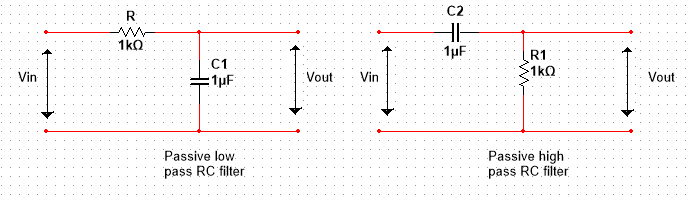
\includegraphics[width=0.70\textwidth]{graphics/passivehighlow.png}
    \caption{Passive low and high pass filters RC filter setups.}
    \label{fig:PassiveHighLow}
\end{figure}

Operational amplifiers or op-amps are devices that amplify voltage signals.
These devices are heavily used in all kinds of signal conditioning and filtering.
The gain of op-amps is a ratio between the input voltage and the output voltage. 

\begin{equation}
    A_v = \frac{V{out}}{V{in}} = 1 + \frac{R_f}{R_{in}}
    \label{eq:DCGain}
\end{equation}

The gain from a non inverting op amp can be found by \textit{Equation \ref{eq:DCGain}}, $A_v$ is the gain and $R_f$ and $R_{in}$ are the resistor values of the resistor configuration seen on the right hand side in \textit{Figure \ref{fig:invNonInvOPamp}}.


\begin{equation}
    A_v = -\frac{V{out}}{V{in}} = -\frac{R_f}{R_{in}}
    \label{eq:invertDCGain}
\end{equation}

The gain from an inverting op amp can be found by \textit{Equation \ref{eq:invertDCGain}}, $A_v$ is the gain and $R_f$ and $R_{in}$ are the resistor values of the resistor configuration seen on the left hand side in \textit{Figure \ref{fig:invNonInvOPamp}}.

\begin{figure}[h]
    \centering
    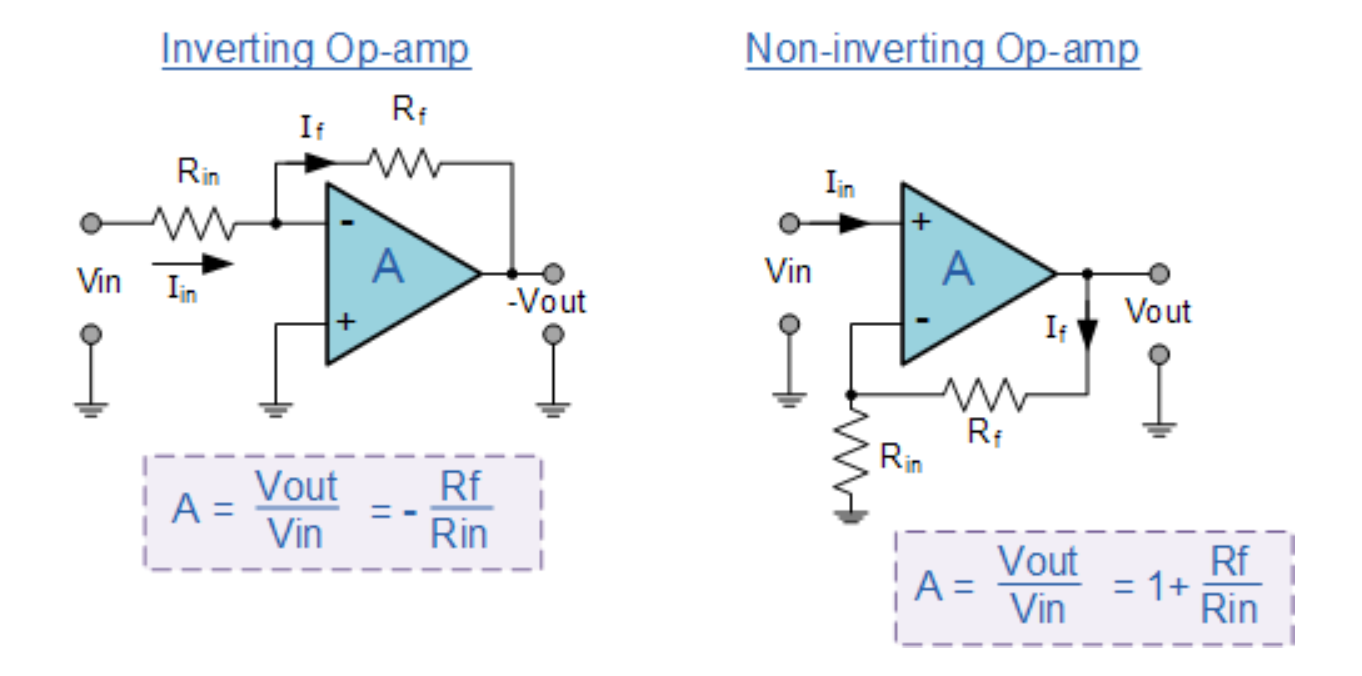
\includegraphics[width=0.70\textwidth]{graphics/invNoninv.png}
    \caption{Inverting and non inverting op amp setups \cite{noauthor_operational_2013}.}
    \label{fig:invNonInvOPamp}
\end{figure}

When the RC filter and op-amps are combined, they form what is called an active filter.
Examples of which can be seen in \textit{Figures \ref{fig:LowPassFilter},\ref{fig:HighPassFiler}} and their respective frequency and phase shift responses in \textit{Figures \ref{fig:LowPassResponse},\ref{fig:HighPassResponse}}.
These filters perform the same as an RC filter in terms of its operations and frequency response with the addition of gain control \cite{noauthor_active_2013-1}.


\begin{equation}
    A_f = \frac{V{out}}{V{in}} = \frac{A_v}{\sqrt{1 + (\frac{f}{f_c})^2}}
    \label{eq:ActiveLowPass}
\end{equation}


The gain of the first order active low pass filter can be found using \textit{Equation \ref{eq:ActiveLowPass}}.
Where $A_f$ is the voltage gain, $A_v$ is the gain seen in \textit{Equation \ref{eq:DCGain}}, f is the frequency of the signal and $F_c$ is the set cutoff frequency.
This has the effect of active gain control depending on the frequency of the input.
When,
\begin{enumerate}
    \item $f < F_c$, $A_f \approx A_v$
    \item $f = F_c$, $A_f = \frac{A_v}{\sqrt{2}} = 0.707 A_v$
    \item$f > F_c$, $A_f < A_v$
\end{enumerate}

\begin{figure}[h]
    \centering
    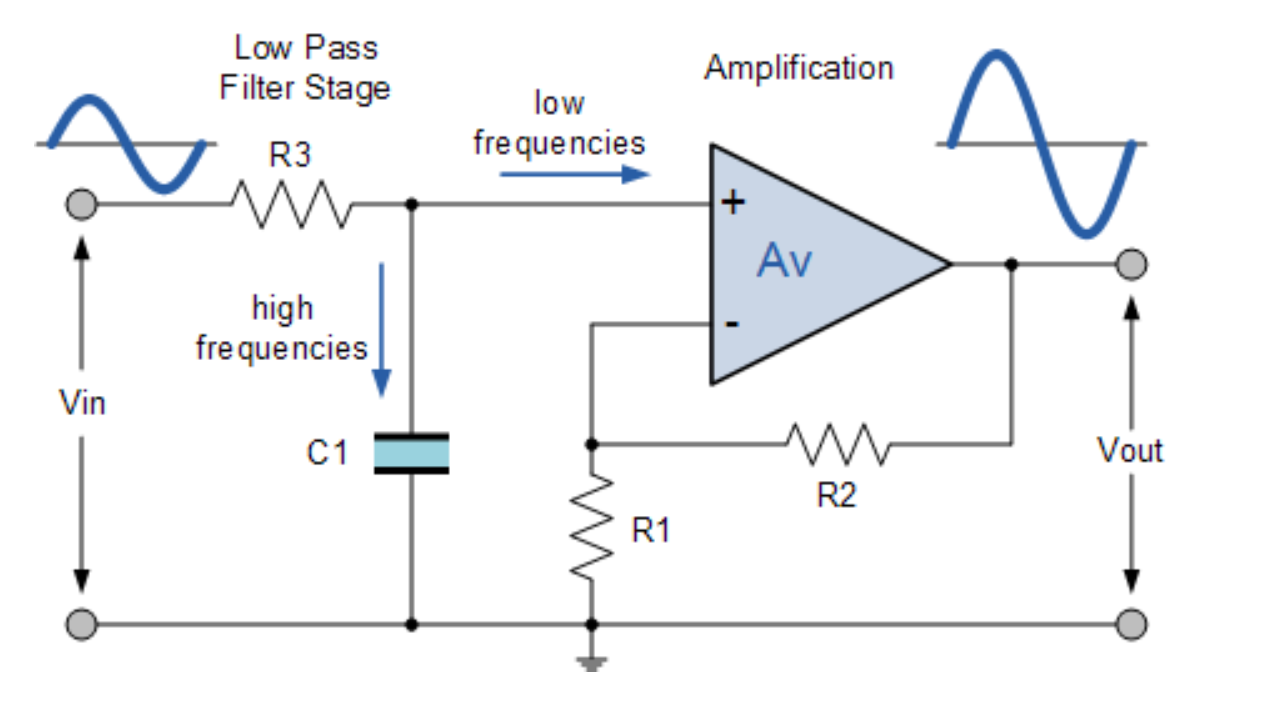
\includegraphics[width=0.70\textwidth]{graphics/lowPassFilter.png}
    \caption{Active first order low pass filter \cite{noauthor_active_2013-1}.}
    \label{fig:LowPassFilter}
\end{figure}

\begin{figure}[h]
    \centering
    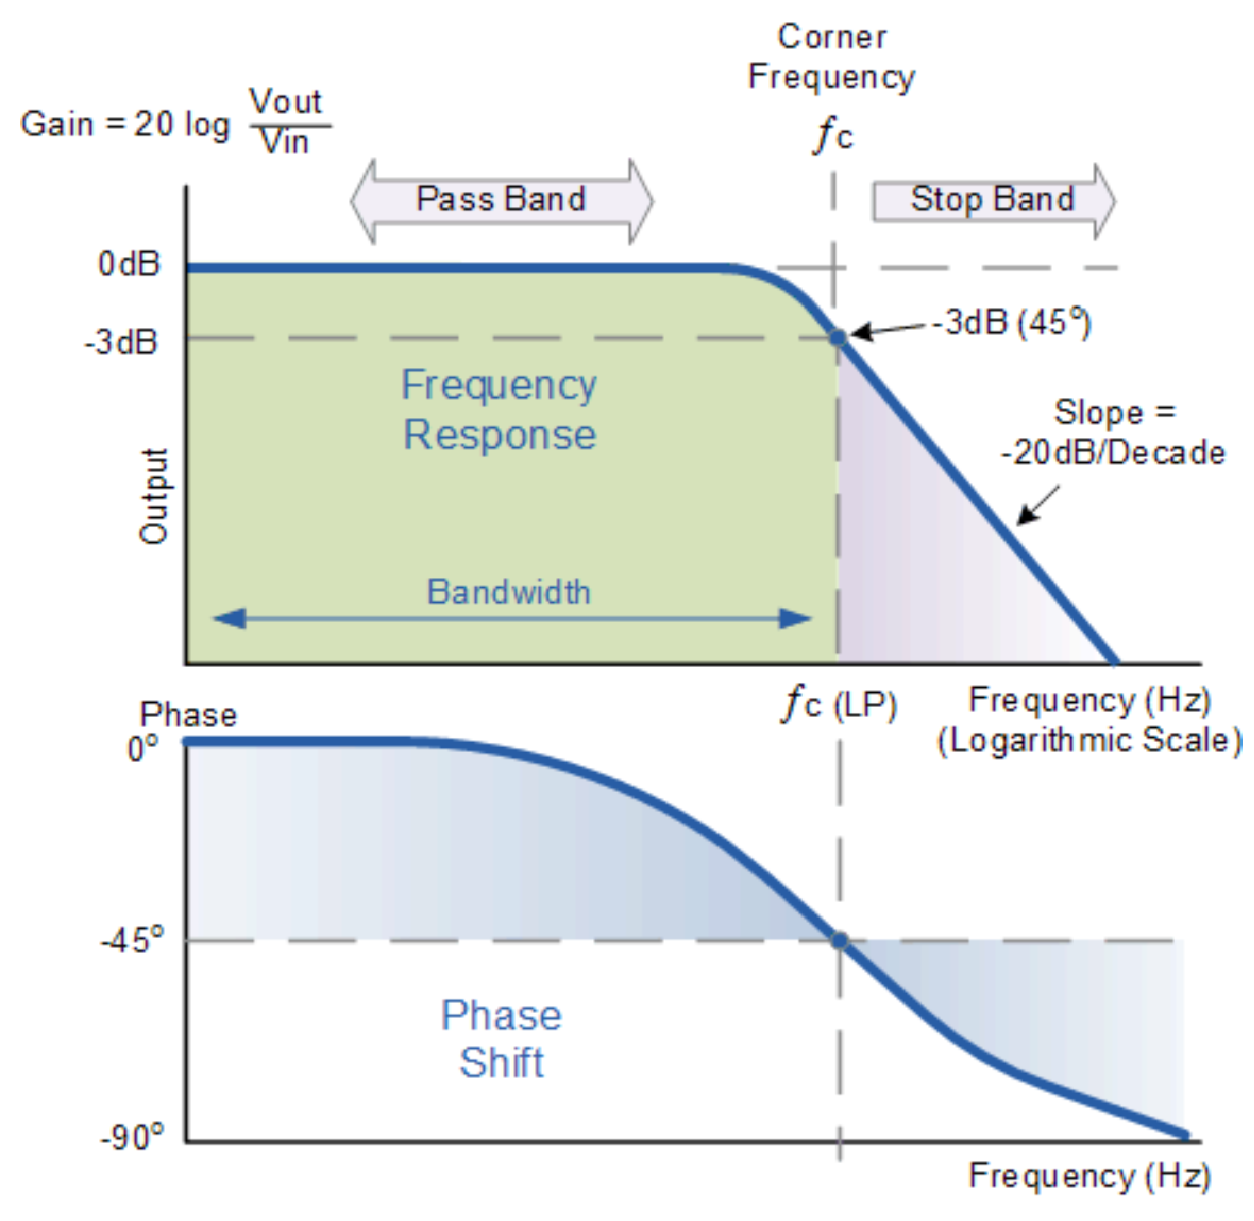
\includegraphics[width=0.70\textwidth]{graphics/lowPassResponse.png}
    \caption{First order RC low pass frequency response and phase shift \cite{noauthor_low_2013}}
    \label{fig:LowPassResponse}
\end{figure}


\begin{equation}
    A_f = \frac{V{out}}{V{in}} = \frac{A_v(\frac{f}{f_c})}{\sqrt{1 + (\frac{f}{f_c})^2}}
    \label{eq:ActiveHighPass}
\end{equation}

The gain of the first order active high pass filter can be found using \textit{Equation \ref{eq:ActiveHighPass}}.
Where $A_f$ is the voltage gain, $A_v$ is the gain seen in \textit{Equation \ref{eq:DCGain}}, f is the frequency of the signal and $F_c$ is the set cutoff frequency.
This has the effect of active gain control depending on the frequency of the input.
When,
\begin{enumerate}
    \item $f < F_c$, $A_f < A_v$
    \item $f = F_c$, $A_f = \frac{A_v}{\sqrt{2}} = 0.707 A_v$
    \item$f > F_c$, $A_f \approx A_v$
\end{enumerate}


\begin{figure}[h]
    \centering
    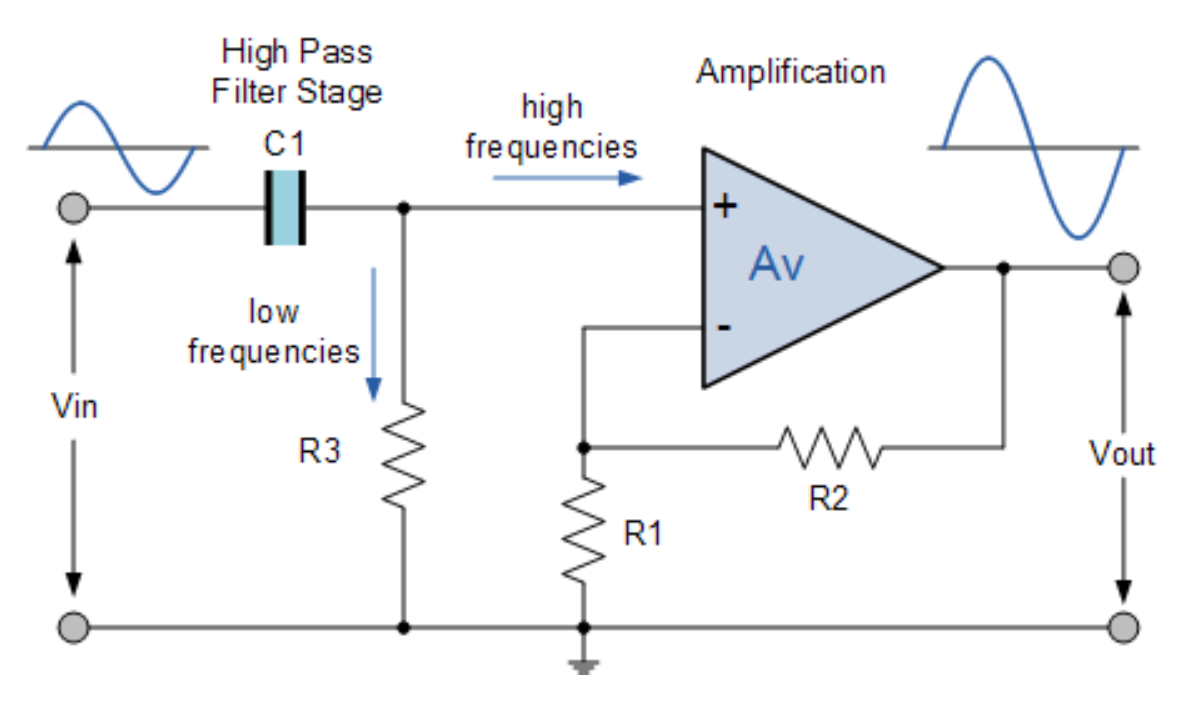
\includegraphics[width=0.60\textwidth]{graphics/highPassFilter.png}
    \caption{Active first order low pass filter \cite{noauthor_active_2013}.}
    \label{fig:HighPassFiler}
\end{figure}

\begin{figure}[h]
    \centering
    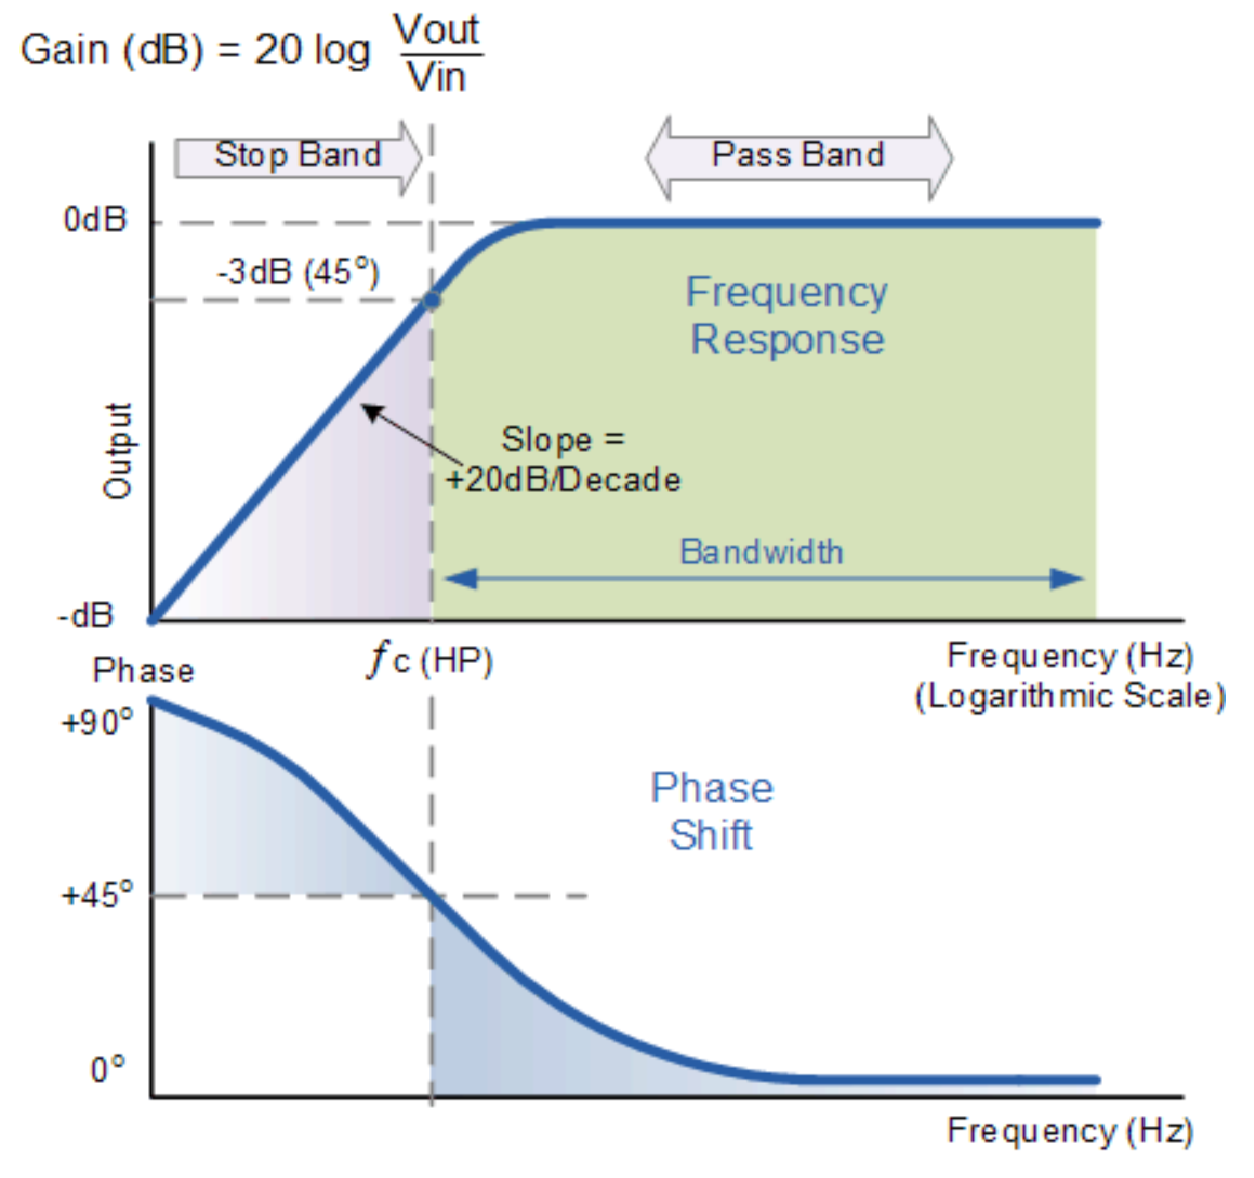
\includegraphics[width=0.60\textwidth]{graphics/highPassResponse.png}
    \caption{First order RC high pass frequency response and phase shift \cite{noauthor_high_2013}}
    \label{fig:HighPassResponse}
\end{figure}

\clearpage

Decibel is a relative unit of measure, used in electronic circuits to express the input values to output value on a logarithmic scale.  

\begin{equation}
    dB = 20log\frac{V{out}}{V{in}}
    \label{eq:DBGAIN}
\end{equation}

The gain in decibel is found by \textit{Equation \ref{eq:DBGAIN}}, where $V{out}$ is the output root mean square (RMS) voltage of the circuit and V{in} is the input RMS voltage.

Summing amplifiers or summing inverter circuits are useful when combining two or more signals together.
An example of the circuit can be seen in \textit{Figure \ref{fig:SummingOpAmp}}, where $R_1 = R_2 = R_3$ would be the same value.
The circuit yields a voltage output that is equal to all the input voltages summed together and multiplied with the unity gain of the amplifier.
This is possible due to the virtual ground that is created by a non-inverting op-amp configuration\cite{noauthor_summing_2013}. 
This circuit is especially useful when there is a need to shift an oscillating AC voltage to have a DC voltage offset.


\begin{figure}[h]
    \centering
    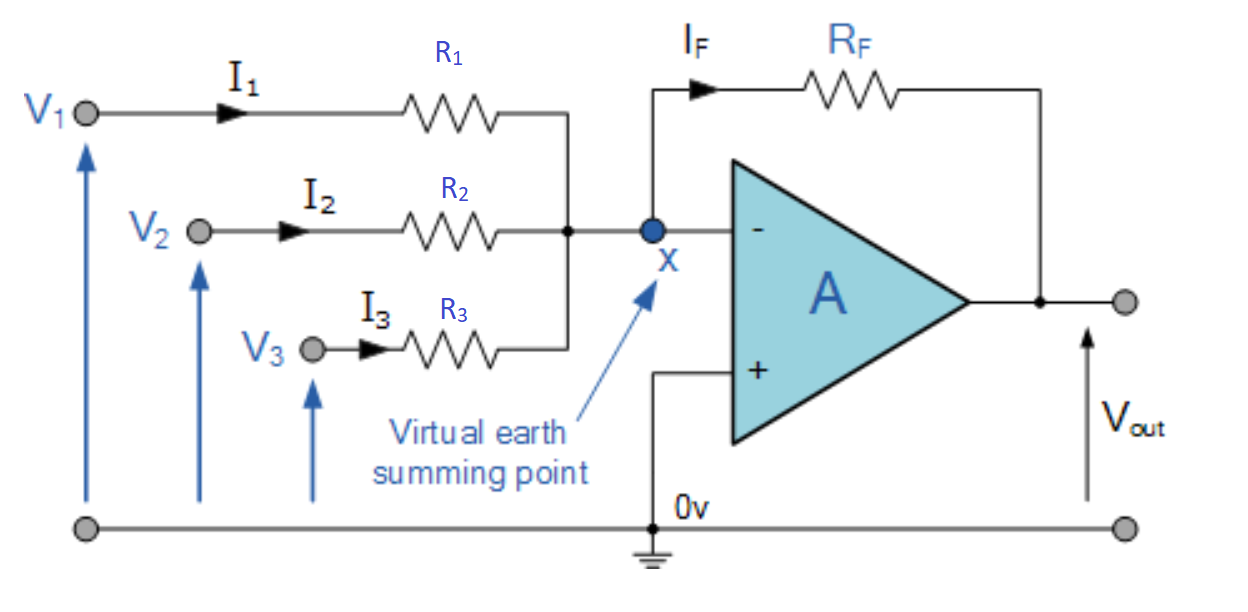
\includegraphics[width=0.70\textwidth]{graphics/SummingOpAmp.png}
    \caption{Scaling summing amplifier circuit \cite{noauthor_summing_2013}}
    \label{fig:SummingOpAmp}
\end{figure}

Scaling summing amplifiers are in the same configuration as summing amplifiers with one main difference which is that resistor values are not equal to one another.
This enables individual scaling of each signal, which means that each input signal can have different gain values.

%$$I_F = I_1 + I_2 + I_3 = -[\frac{V_1}{R_{1}} + \frac{V_2}{R_{2}} + \frac{V_3}{R_{3}}]$$
%$$-V_{out} = \frac{R_F}{R_{1}}V_1 +\frac{R_F}{R_{2}}V_2 +\frac{R_F}{R_{3}}V_3$$

\begin{equation}
    V_{out} = -R_F(\frac{V_1}{R_{1}} +\frac{V_2}{R_{2}} +\frac{V_3}{R_{3}} + ...)
    \label{eq:ScalingGain}
\end{equation}

Finding the output voltage can be found using \textit{Equation \ref{eq:ScalingGain}}.
Where $V_out$ is the output voltage, $R_f$ is the voltage across the input and output of the op-amp, $R_1, R_2$ and $R_3$ are the resistor value of the different input signals.
Let's take for an example of an AC signal that needs to be shifted so that there is no negative voltage, see \textit{Figure \ref{fig:sumCircuitexamp}} for the layout of the circuit.
The AC signal (U1B\_out) would along with the shifting signal, in this case a DC voltage of 1.65V.
The AC signal is scaled by a factor of A = $\frac{180\Omega}{90\Omega}$ = 2.
How ever the DC voltage signal only scaled by a factor of A = $\frac{180\Omega}{180\Omega}$ = 1.
The voltage output, U1C\_out can be seen in \textit{Figure \ref{fig:SummingOpAmpShift}} as the red signal and the input signal, U1B\_out is represented by the white signal.
This creates a problem though, the output signal is shifted by $90\deg$ and the scaling op-amp is in an inverting configuration the signal is inverted, so it is negative.
Both are fixed by the addition of U1D, an inverting amplifier.
This puts the signal back in phase with the original input signal as well as it now is positive, as seen in \textit{Figure \ref{fig:SummingOpAmpShift1}} where the red signal is U1D\_out the output of the inverting amplifier and the white signal is the original input signal U1B\_out.


\begin{figure}[h]
    \centering
    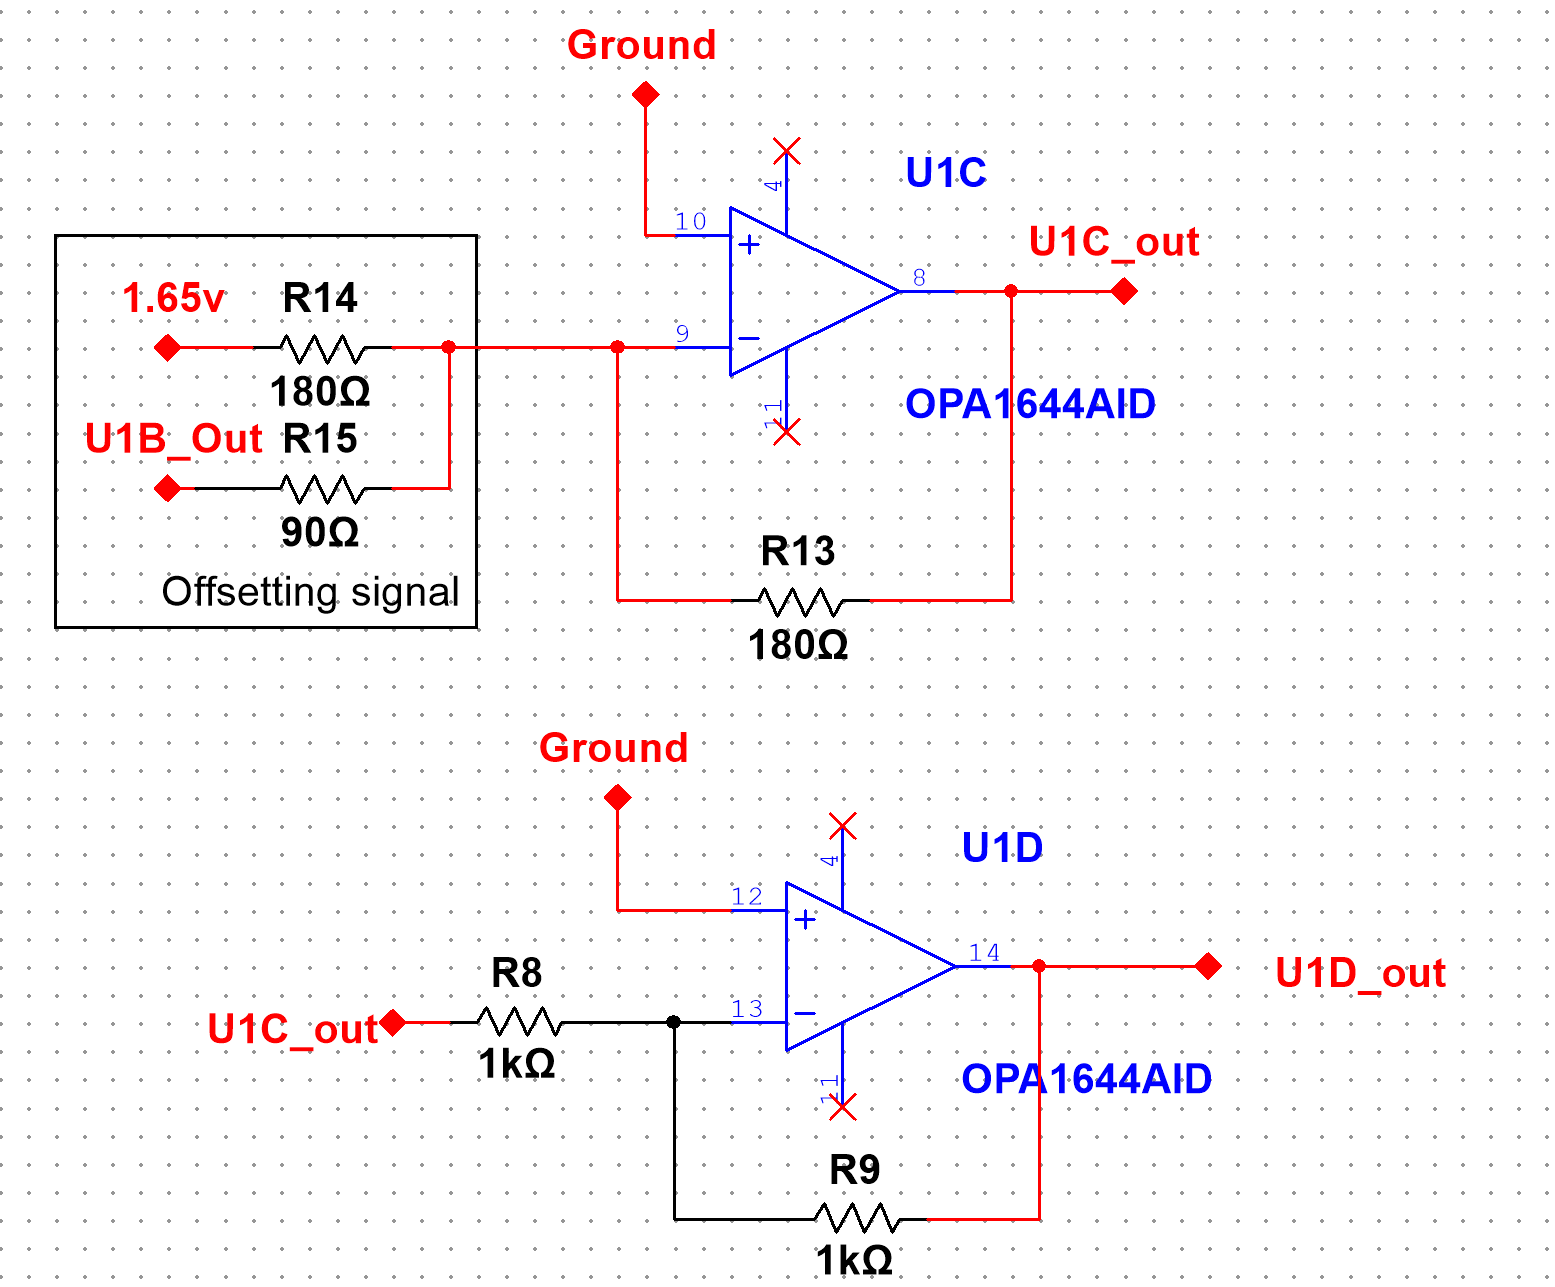
\includegraphics[width=0.70\textwidth]{graphics/sumCircuitexamp.png}
    \caption{Example of a scaling amplifier circuit where two signals are combined to create a shift of the original signal. U1C represents the scaling amplifier, U1D is a normal inverting amplifier.}
    \label{fig:sumCircuitexamp}
\end{figure}

\begin{figure}[h]
    \centering
    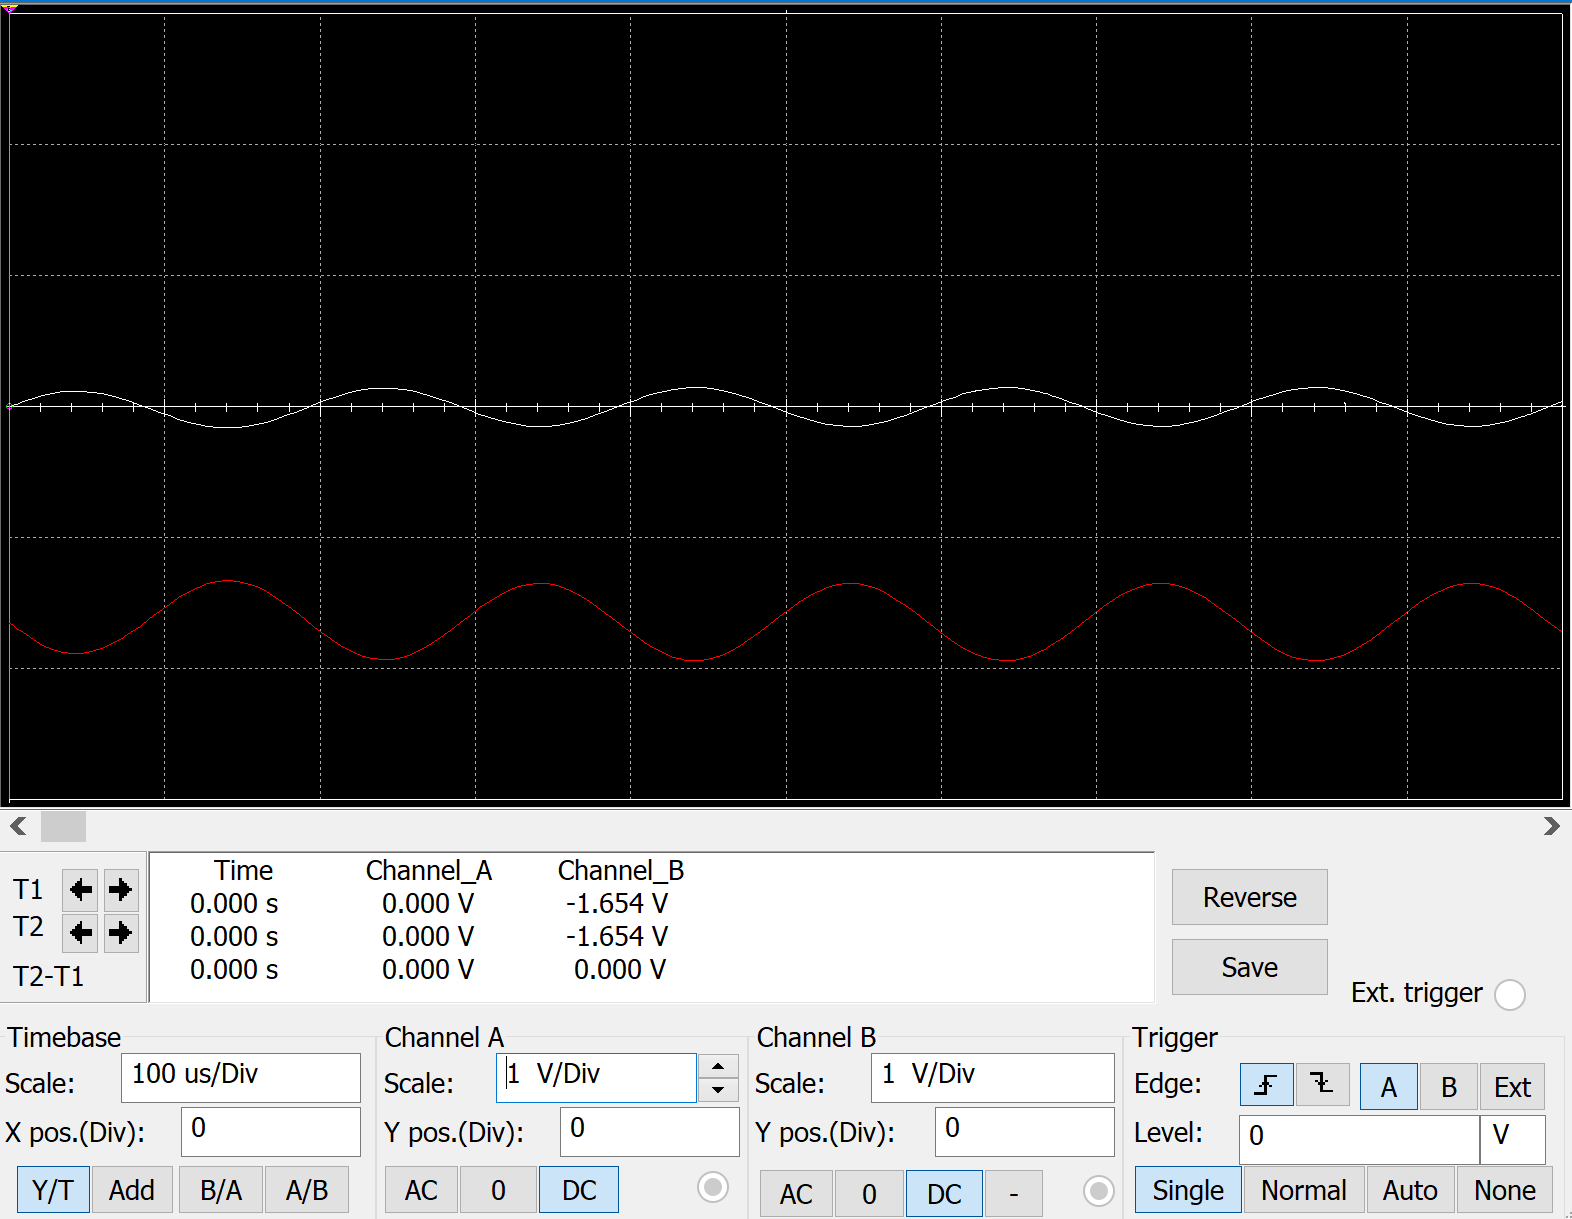
\includegraphics[width=0.70\textwidth]{graphics/summingShift.png}
    \caption{Example of the signal shift of a summing Op Amp circuit, the red signal represents the voltage output U1C\_out and the white signal is the input AC signal U1B\_out.}
    \label{fig:SummingOpAmpShift}
\end{figure}

\begin{figure}[h]
    \centering
    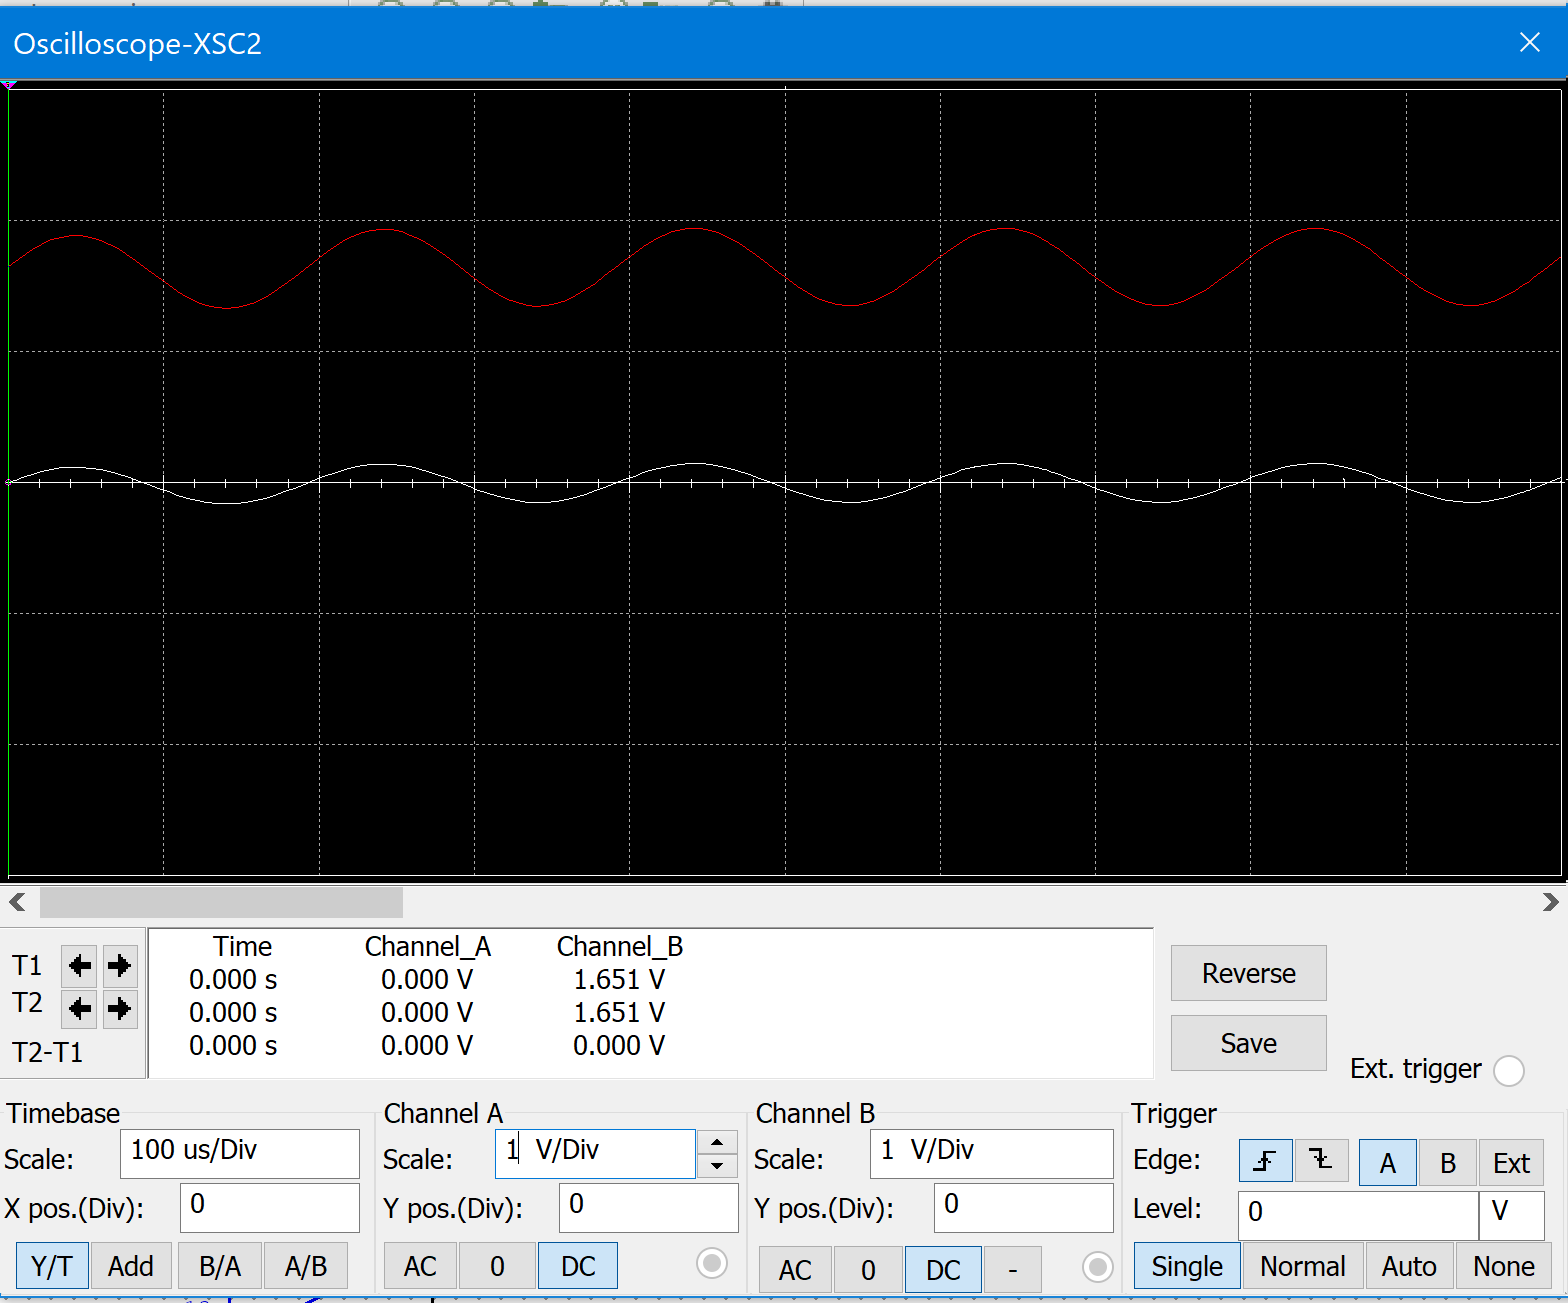
\includegraphics[width=0.70\textwidth]{graphics/summingShift1.png}
    \caption{Example of the signal shift of a summing Op Amp circuit, the red signal represents the voltage output U1D\_out and the white signal is the input AC signal U1B\_out}
    \label{fig:SummingOpAmpShift1}
\end{figure}


\clearpage

%\fxfatal{SKOÐA H'ER-----------------------}
%ADC CHARECTERISTICS https://forum.pjrc.com/threads/44929-Teensy-3-5-ADC-characteristcs
%SD POSSIBLE https://forum.pjrc.com/threads/45993-Teensy-3-6-ADC-DMA-Question
%Teensy36ISRLogger Skilar með 8gb kortinu 6.67MB/s
%https://forum.pjrc.com/threads/49975-writing-binary-file-on-SD-card-in-Teency-3-5

\subsection{Microcontroller/Microcomputer}%Breyta um titil

%For this project the most important factors when choosing a microcontroller/microcomputer were regarding the ADC specifications as well as the power consumption.%\fxfatal{VITNA Í GOALS} tala um upplausn bit, power og fleira

\subsubsection{Arduino}

Arduino Uno is a programmable board that uses the 8-bit ATmega328p microcontroller.
Which is probably one of the most popular microcontroller in the world and the Arduino board is one of them and is among the best beginner boards to use because of the shear amount of documentation and tutorials for it.
The microcontroller main features can be seen in \textit{Table \ref{Tab:ATmega328p}}.


\begin{figure}[h]
    \centering
    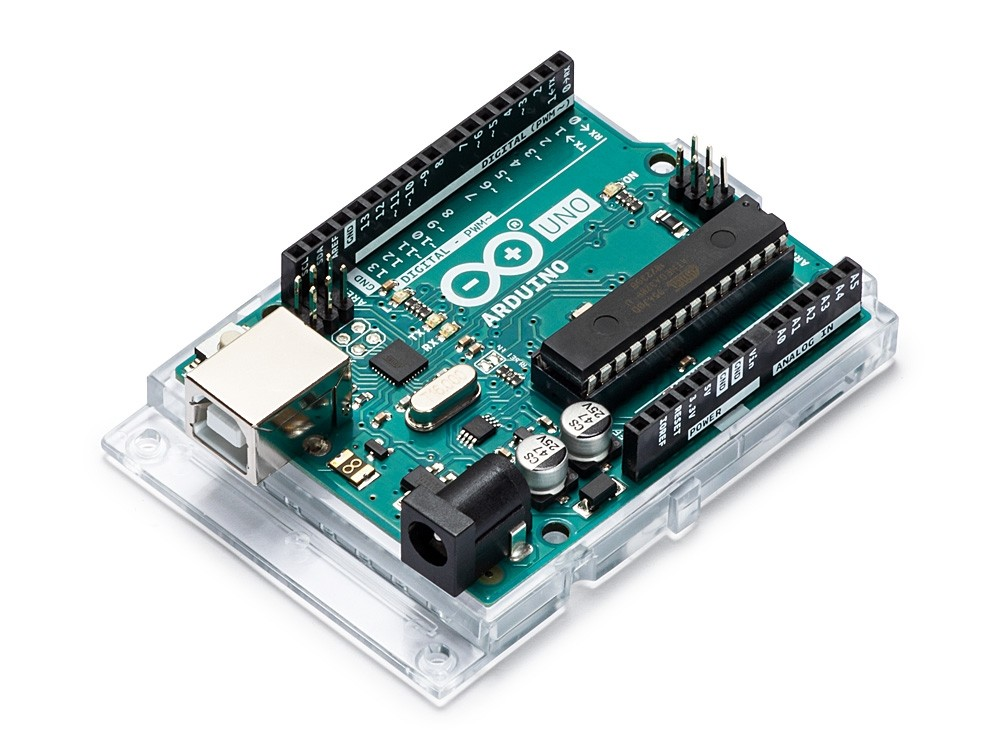
\includegraphics[width=0.70\textwidth]{graphics/ArduinoUNo.jpg}
    \caption{The Arduino Uno \cite{noauthor_arduino_nodate}}
    \label{fig:Arduino}
\end{figure}

\begin{table}[h]\caption{Main features of the ATmega328p \cite{noauthor_atmega328p_nodate}}.\label{Tab:ATmega328p}
\centering
    \begin{tabular}{|l|l|}
    \hline
        Parameters                        & Value                \\ \hline
        Flash memory [KB]                 & 32                      \\ \hline
        ADC resolution [bit]              & 10                   \\ \hline
        ADC sample speed [ksps]           & 15                     \\ \hline
        Digital Communication Peripherals & 1-UART, 2-SPI, 1-I2C \\ \hline
        Operating Voltage [V]             & 1.8 to 5.5           \\ \hline
        Max power consumption [W]         & 0.66               \\ \hline
        Price                             & 33\$                \\ \hline
    \end{tabular}
\end{table}


The Arduino has 14 digital input/output (I/O), and 6 can be used as pulse width modulation (PWM) outputs as well as 6 analog inputs.
The board has a USB connector which the board is programmed through as well as power it.
Arduino also provides its users with a free open-source Arduino software integrated development environment (IDE).  \cite{noauthor_arduino_nodate}.
As well as a 6-channel 10-bit resolution ADC and up to 15 kilo samples per second (ksps).
The board has a maximum current draw of 200mA, so at an operating voltage of 3.3V, the power consumption is at most 0.66W\cite{noauthor_atmega328p_nodate}.


\subsubsection{Raspberry Pi}

Unlike the Arduino, the Raspberry Pi is not only a programmable microcontroller but rather a single-board microcomputer and is the third most sold computer brand worldwide \cite{noauthor_faqs_nodate}.
Currently, there are 13 different models of the Raspberry Pi's with varying pricing and capabilities some of which can be seen in \textit{Table \ref{Tab:RaspbModel}}. 
Raspberry Pis can be used with several operating systems for instance Linux, FreeBSD or a Raspberry pi OS that can come with or without a desktop.

\begin{center}
\begin{table}[h]\caption{Comparison of different Raspberry Pi models\cite{noauthor_faqs_nodate}}.\label{Tab:RaspbModel}
    \begin{tabular}{|l|l|l|l|c|}
    \hline
    \textbf{\begin{tabular}[c]{@{}l@{}}Raspberry Pi\\ Product\end{tabular}}        & \textbf{SoC} & \textbf{Speed} &  \textbf{\begin{tabular}[c]{@{}l@{}}Recommended\\ power supply \\ current capacity\end{tabular}} & \textbf{\begin{tabular}[c]{@{}l@{}}Typical bare-\\board current \\ consumption\end{tabular}} \\ \hline
     Model A+   & BCM2835      & 700MHz         & 0.7A          & 0.2A            \\ \hline
     Model B+   & BCM2835      & 700MHz         & 1.8A          & 0.33A            \\ \hline
     2 Model B  & BCM2836/7    & 900MHz         & 1.8A          & 0.5A                 \\ \hline
     3 Model B  & BCM2837A0/B0 & 1200MHz        & 2.5A          & 0.4A                  \\ \hline
     3 Model A+ & BCM2837B0    & 1400MHz        & 2.5A          & 0.35A                  \\ \hline
     3 Model B+ & BCM2837B0    & 1400MHz        & 2.5A          & 0.5A                  \\ \hline
     4 Model B  & BCM2711      & 1500MHz        & 3.0A          & 0.6A                  \\ \hline
     Zero       & BCM2835      & 1000MHz        & 1.2A          & 0.1A                   \\ \hline
     Zero W     & BCM2835      & 1000MHz        & 1.2A          & 0.15                  \\ \hline
     Zero WH    & BCM2835      & 1000MHz        & 1.2A          & 0.15                  \\ \hline
     400        & BCM2711      & 1800MHz        & 3.0A          & 0.8A                  \\ \hline
    \end{tabular}
\end{table}
\end{center}

Raspberry recommends powering the Raspberry Pi using 5V.
This means that the Raspberry Pi uses quite a bit of power, Raspberry Pi Zero (6W) Raspberry Pi 2 B (9W), Raspberry Pi 3(12.5W).
Taking a closer look at the Raspberry Pi Zero since it fits within the power consumption specifications.
The microcomputer costs around 30 \$, has a 1GHz single-core CPU, 512MB RAM, Mini HDMI port, Micro USB OTG port,
Micro USB power and HAT-compatible 40-pin header.
It has i2c, SPI, PWM and serial pins, all GPIO pins are digital and can be configured to be input or output pins.
which can be seen in \textit{Figure \ref{fig:RPIGPIO}}.

\begin{figure}[h]
    \centering
    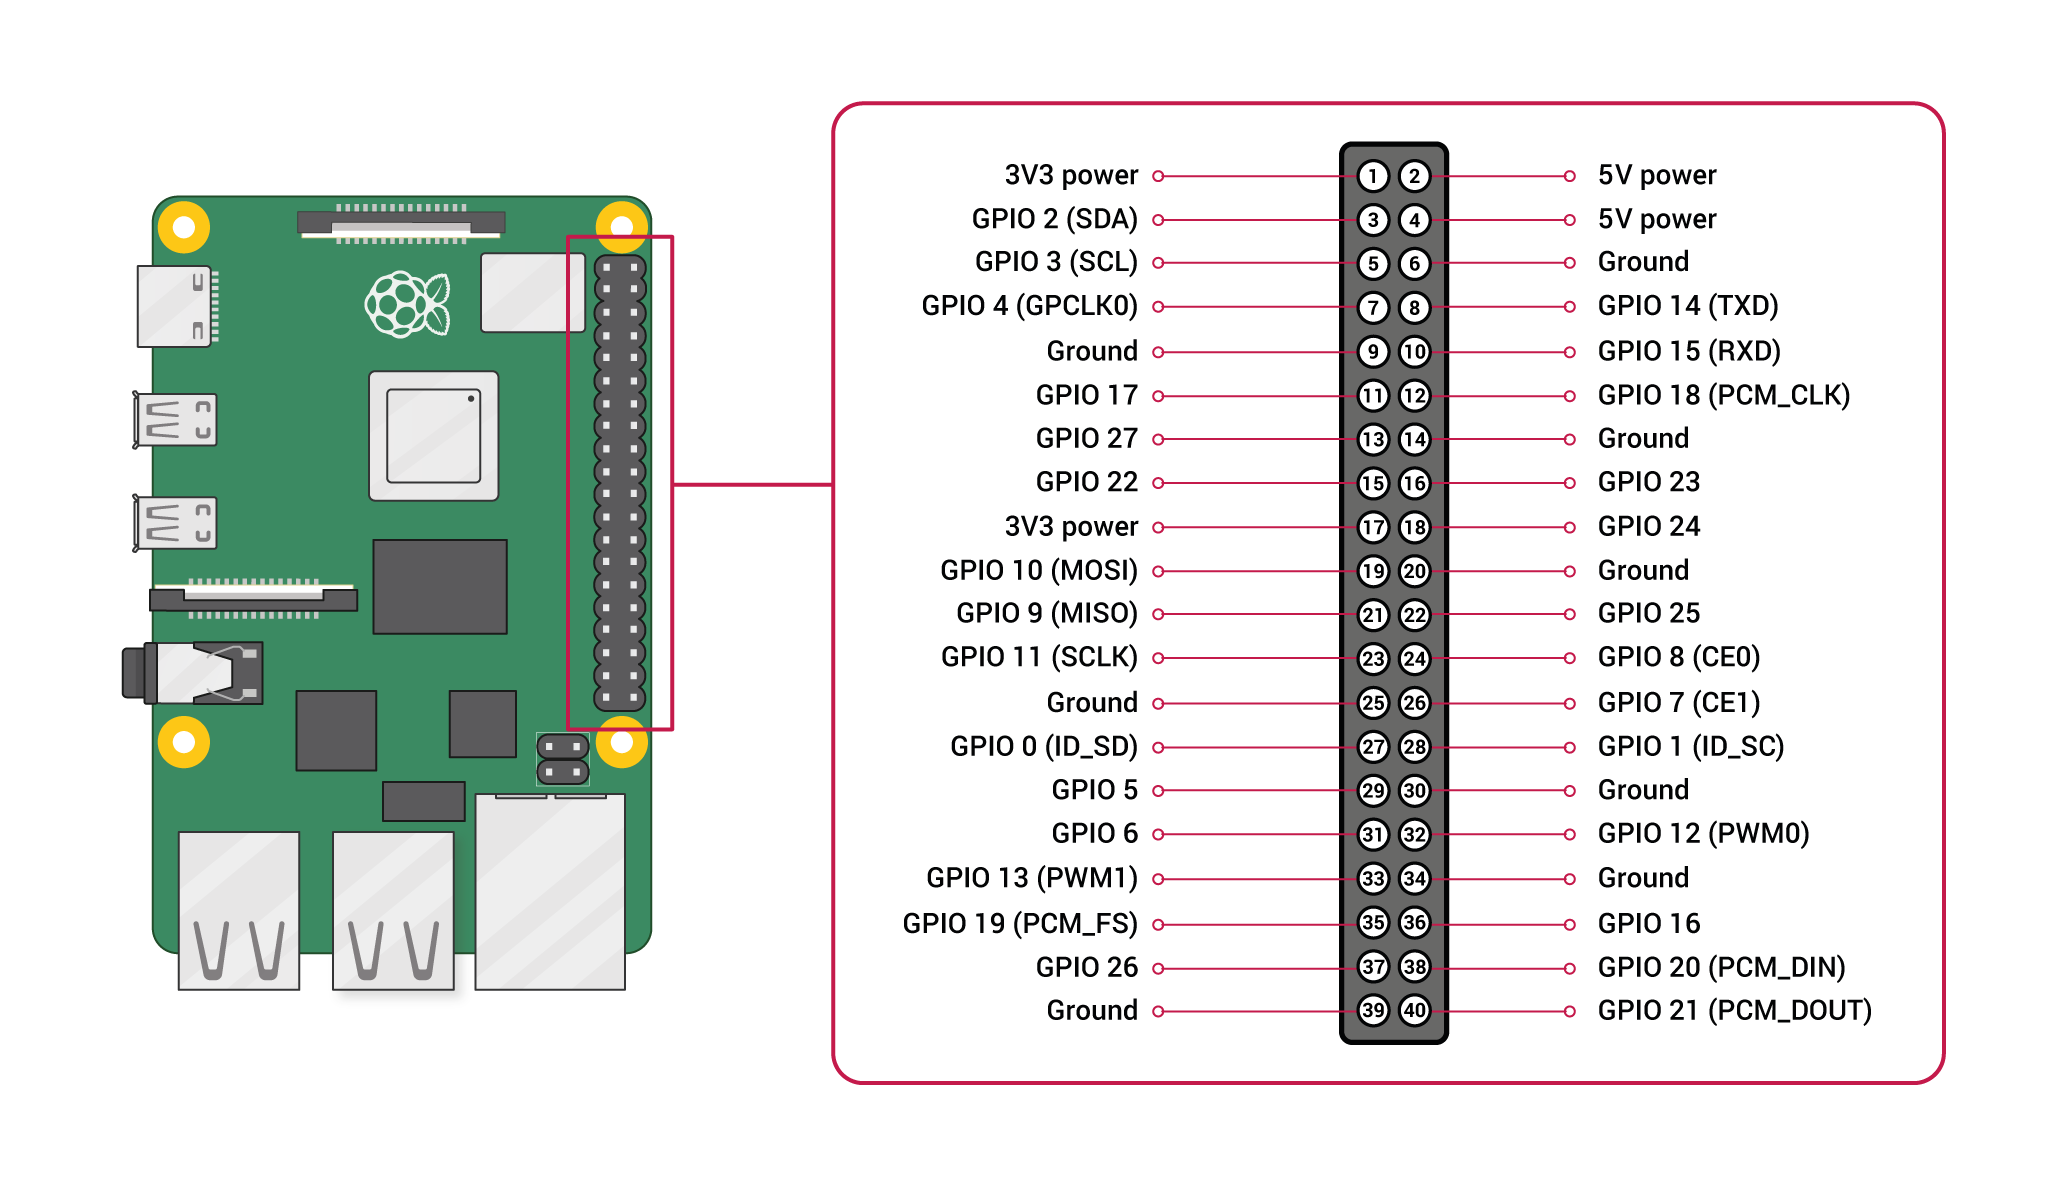
\includegraphics[width=0.70\textwidth]{graphics/ZeroGPIO.png}
    \caption{GPIO of the Raspberry Pi Zero \cite{noauthor_gpio_nodate}}
    \label{fig:RPIGPIO}
\end{figure}

The Raspberry Pi is also limited in the fact that it has no analog I/O pins, meaning that it can not convert analog to digital signals on its own.
However, there is a way to record audio, which is done through a sound card.
Several solutions have already been made available for this such as the Audio Injector stereo sound card which can directly connect to the general purpose input output (GPIO) pins of Raspberry Pi2, Pi3 and Pi Zero.
The card is made for an electret microphone and can supply the Raspberries with input and output audio.
The card has stereo RCA input and output, a headphone jack and a preamplifier, a volume knob and a low latency of 540 $\mu$s for both the input and output \cite{noauthor_rpi_nodate}.

\begin{figure}[h]
    \centering
    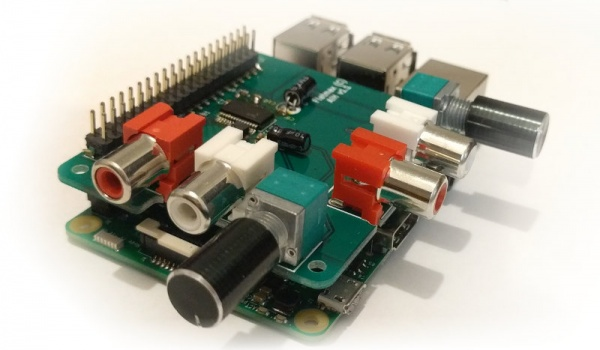
\includegraphics[width=0.70\textwidth]{graphics/rpisoundcard.jpg}
    \caption{The Audio Injector stereo sound card \cite{noauthor_rpi_nodate}}
    \label{fig:rpisoundcard}
\end{figure}


\subsubsection{Teensy}

Teensy's are the same as Arduino's as being a USB programmable single-board microcontroller.
The boards are can be programmed with multiple programs such as the Arduino IDE software and can use both the examples and libraries that come with the program.
This is possible through an addition called Teensyduino which also includes a large library for programming.
Other programs include Visual Micro, which enables programming on Visual Studio Code, PlaformIO IDE and CircuitPython (only available on Teensy 4.X) which allows python programming.
There are multiple models available, ranging in price, size and capabilities as seen in \textit{Table \ref{Tab:TeensyModel}}.


\begin{table}[h]\caption{Comparison of different Teensy models\cite{noauthor_teensy_nodate}}.\label{Tab:TeensyModel}
\begin{tabular}{|l|l|l|l|l|}
\hline
\multicolumn{1}{|c|}{\textbf{Specification}} & \multicolumn{1}{c|}{\textbf{Teensy 2.0}}                               & \multicolumn{1}{c|}{\textbf{Teensy 3.0}}                                            & \multicolumn{1}{c|}{\textbf{Teensy 3.5}}                                                  & \multicolumn{1}{c|}{\textbf{Teensy 4.1}}                                              \\ \hline
Processor & \begin{tabular}[c]{@{}l@{}}ATMEGA32U4\\ 8 bit AVR\\ 16 MHz\end{tabular} & \begin{tabular}[c]{@{}l@{}}MK20DX128\\ 32 bit ARM\\ Cortex-M4\\ 48 MHz\end{tabular} & \begin{tabular}[c]{@{}l@{}}MK64FX51\\2VMD12\\ 32-bit ARM\\ Cortex- M4\\ 120MHz\end{tabular} & \begin{tabular}[c]{@{}l@{}}MIMXRT1062\\ 32 bit ARM\\ Cortex-M7\\ 600 MHz\end{tabular} \\ \hline
\begin{tabular}[c]{@{}l@{}}Flash Memory\\ {[KB]}\end{tabular} & 32 & 131 & 512 & 7936 \\ \hline
%\begin{tabular}[c]{@{}l@{}}RAM Memory\\ (Bytes)\end{tabular}& 2560 & 16384 & 256K & 1024K \\ \hline
%\begin{tabular}[c]{@{}l@{}}EEPROM\\ (Bytes)\end{tabular} & 1024 & 2048 & 4096 & 4096 \\ \hline
\begin{tabular}[c]{@{}l@{}}Direct Memory\\ Access [Channels]\end{tabular}  & - & 16 & 16 & 32 \\ \hline
%I/O [Pins, V] & 25, 5 Volt & 34, 3.3 V & \begin{tabular}[c]{@{}l@{}}64, 3.3V,\\ 5V tol\end{tabular} &\begin{tabular}[c]{@{}l@{}}55, 3.3V,\\ 5V tol\end{tabular}   \\ \hline
\begin{tabular}[c]{@{}l@{}}ADC resolution\\ {[bit]}\end{tabular} & 10 & 16 & 16   & 12     \\ \hline
%PWM & 7 & 10 & 20 & 35 \\ \hline
UART,I2C,SPI & 1,1,1 & 3,1,1 & 6,3,3 & 8,3,3 \\ \hline
Price [\$] & {16.00} & {19.00} & {24.25} & {26.85} \\ \hline
\end{tabular}
\end{table}

Taking a closer look at the comparison between the Teensy 3.5 and the Teensy 4.1.
Teensy 3.5 has 2 16bit, 416 ksps (in 16-bit mode) and 818.3 ksps for (<= 13-bit mode), 12MHz ADC\cite{freescale_semiconductor_kinetis_2021-1} and has a voltage range of 0-3.3V, as well as some are 5V tolerant while the Teensy 4.1 offers 12 bits of resolution and 20MHz (samples per second is not specified) and a range of 0 - 3.3V.
%The Teensy 3.5 also has an option of using pins connected to differential amplifiers, which can decrease unwanted noise of input analog signals.
%Teensy 3.5 also has two digital to analog converters (DACs) output.
%Which makes it capable of outputting audio signals.
Both Teensy's have a voltage regulator which reduces the 5V VUSB / VIN power to 3.3V for use by the main processor and most other parts. Additional circuitry may be powered from the 3.3V pin.
The recommended maximum for external 3.3V usage is 250mA or 0.825W.
When Teensy 3.5 is running at 120MHz processor speed it consumes roughly 50mA at 5V or 0.25W.
While the Teensy 4.0 consumes roughly 100mA at 5V or 0.5W at 600MHz processor speed.
%When power is not applied to VUSB or VIN, it is however possible to run by externally applying 3.3V power.
%There are two ways to power the Teensy's, the first one is to power them via USB.
%The Teensy is equipped with a voltage regulator which regulates the USB voltage of 5V down to 3.3V.
%They can also be powered straight to a VIN pin, which is recommended as a maximum of 3.3V and a 250mA %draw.
\cite{noauthor_teensy_nodate-1}%4.1
\cite{noauthor_teensy_nodate-2}.%3.5

%%% Local Variables: 
%%% mode: latex
%%% TeX-master: "DEGREE-NAME-YEAR"
%%% End: 
